\documentclass[a4paper,onecolumn,11pt]{report}

% Use for onecolumn layout
\usepackage[left=3cm,right=3cm,top=3cm,bottom=3cm]{geometry}

\usepackage{setspace}
\onehalfspace

\usepackage{graphicx}
\usepackage{caption}
\usepackage{subcaption}

\usepackage{listings}

\lstset{ %
  basicstyle=\footnotesize\ttfamily %
}

\usepackage[utf8]{inputenc}
\usepackage[hyphens]{url}

\usepackage{natbib}
\usepackage{textcomp}
\usepackage[greek,english]{babel}
\usepackage{amsmath}

\usepackage{physics}

\frenchspacing
%\renewcommand{\thefootnote}{\alph{footnote}}
\hyphenation{LeVeque}

\begingroup
\lccode`\~=`\ %
\lowercase{%
  \gdef\assignment{\setcounter{word}{0}%
    \catcode`~=\active
    \def~{\space\stepcounter{word}}}}%
\endgroup
\newcounter{word}
\def\endassignment{\stepcounter{word}%
  \begin{flushright}%
  (\arabic{word} words)%
  \end{flushright}%
}

\newcommand{\eq}[1]{#1^\mathrm{eq}}

\title{Accurate methods for computing rotation-dominated flows }

\author{Martin Büttner, University College London \\ MSci Theoretical Physics \\ \\ Supervisor: Prof. Edward Johnson}
\date{\today}

\begin{document}

\maketitle

%!TEX root = ../final-report.tex
\begin{abstract}

Atmospheric and oceanic flows are often modelled using the Shallow Water Equations (SWEs) with the addition of source terms to account for varying topography and the rotation of the Earth. Naive numerical methods fail to preserve steady states in which these additional effects are large but exactly cancelled by pressure gradients in the system. This is a significant shortcoming, as large-scale real-world flows are usually very close to such a balance at all times. This report investigates two existing methods to obtain so-called \emph{well-balanced} solvers. The author was not able to use one of the methods as presented originally, but was able to derive an alternative formulation which did work. New solvers for the SWEs under rotation have been developed based on these methods and implemented with the software package \emph{Clawpack}. The new solvers were shown to be able to preserve these steady states at least to machine precision.

\end{abstract}

\tableofcontents

%!TEX root = ../final-report.tex
\chapter{Introduction}
\label{ch:introduction}

The shallow water equations (SWEs) are a simplified but very effective model for incompressible fluid flow. Despite the name, this model has been particularly successful in modelling large-scale geophysical flows of atmospheric and oceanic currents --- ``shallow'' refers to the relative vertical and horizontal length scales. Considering flows on the scale of the Earth, which can easily extend across several thousand kilometres, the roughly 4 kilometre deep ocean is indeed comparably shallow.

In the context of these applications, two effects are particularly important to model: the Coriolis force, due to the rotation of the Earth, as well as varying topography\footnote{Undersea topography is usually referred to as \emph{bathymetry}. This term will be used predominantly throughout this report.}. This report is concerned with simulating such models using \emph{finite volume methods}. These will usually include the above effects as source terms. Computational difficulties arise in steady flow when these very large forces balance pressure gradients exactly. This is referred to as a geostrophic balance, and large-scale real-world currents are close to this balance at all times. Therefore, the interest of this report lies in numerical methods which work around these computational problems such that they preserve geostrophic flows exactly and can reliably compute small perturbations of these steady states.

\section{Literature Overview}

The SWEs are a hyperbolic system of conservation laws. A lot of effort has been put into studying and solving these systems of equations numerically. Several textbooks about the numerical methods considered in this report exist, including \citet{leveque1992numerical}, \citet{toro1999riemann} and \citet{leveque2002finite}, as well as \citet{toro2001shock} which focuses on the SWEs in particular. In addition, there is a textbook on the rotating SWEs by \citet{zeitlin2007nonlinear}, Chapter 4 of which focuses on numerical methods.

Such hyperbolic systems can be solved using finite volume methods in which the domain is divided up into a (not necessarily regular) grid of control volumes, and the conserved quantities are discretised by assuming that they are constant across each such volume. Note that ``volume'' is being used in a generalised sense here --- for a two-dimensional system like the SWEs, the grid cells are actually areas. The most popular of these methods is due to \citet{godunov1959difference}\footnote{The author could not obtain an English translation of this Russian paper, but the method developed by Godunov has been extensively reiterated in papers and textbooks. Therefore, the following explanation of the method is based on what the author was able to find in those secondary sources.} and is simply known as Godunov's method --- in fact, today a whole family of Godunov methods has been developed based on the concepts derived in this original paper.

A fairly recent review of Godunov-type methods was conducted by \citet{toro2007godunov} and an older review can be found in \citet{sweby2001godunov}.

The piecewise-constant discretisation reduces the problem to a number of step functions at the cell boundaries. Such an initial-value problem for conservation laws is known as a Riemann problem (see \citet{toro1999riemann}, Section 2.2.2, \citet{leveque2002finite}, Section 3.8, or \citet{toro2007godunov}, Section 2.1) and can be solved exactly for many systems. By solving each of these Riemann problems, the discretised SWEs can be solved. The other insight of Godunov's method is that each hyperbolic system has a number of characteristic waves which only propagate in certain directions at finite speeds, which allows to simplify the computation by only looking at waves that can propagate \emph{into} each cell. This technique is known as \emph{upwinding}.

While it is possible to solve the Riemann problem exactly for many systems (including the SWEs), this dominates the computations required to solve each time step. Therefore, approximate solvers have been developed, the most popular one being due to \citet{roe1981approximate}. See the textbooks mentioned above for an overview of exact and approximate Riemann solvers.

However, these methods generally have been developed for homogeneous systems. A simple approach to account for source terms like bathymetry and the Coriolis force is to compute these independently of the homogeneous system in a separate step. This leads to problems in steady or quasi-steady scenarios, such that the flux terms arising from the homogeneous system and the source terms are balanced at all times. According to \citet{toro2007godunov}, the first authors to recognise this were \citet{glimm1984generalized}. Preserving such a balance, requires that a time step in the homogeneous system is  cancelled exactly by the corresponding time step for the source terms. Since these terms can in principle be very large, even for balanced systems, due to different methods being employed and numerical inaccuracies, this is practically impossible. Hence, equilibria cannot be modelled accurately, even the system is as simple as a still lake. The numerical errors create spurious oscillations which may even be amplified in future time steps. Furthermore, small perturbations away from equilibrium would be completely dominated by said numerical errors. These problems are particularly relevant for large-scale geophysical flows, which are usually very close to geostrophic balance --- an instance of balanced flux and source terms --- at all times.

Therefore, a lot of research was conducted over the past two decades to develop so-called \emph{well-balanced} methods which are able to preserve these equilibria exactly. To the best of the author's knowledge, \citet{greenberg1996well} were the first to use the term ``well-balanced''.

Subsequently, dozens of well-balanced methods have been developed, including \citet{leveque1998balancing}, \citet{garcia2000numerical}, \citet{hubbard2000flux}, \citet{burguete2001efficient}, \citet{gascon2001construction}, \citet{rogers2001adaptive}, \citet{bale2003wave}, \citet{rogers2003mathematical}, \citet{audusse2004fast}, \citet{chinnayya2004well}, \citet{liang2009adaptive}, \citet{liang2009numerical}. The most recent articles the author could find are by \citet{zhang2014well} and \citet{chertockwell}, the latter being of particular relevance here, as their assumptions align with those made in this report. Furthermore, Section 4.4 of \citet{zeitlin2007nonlinear} presents a long list of other well-balanced methods applicable to the rotating SWEs and refers to the method discussed in \citet{audusse2004fast} and related works as ``the most classical [well-balanced] method''. With \citet{bouchut2004nonlinear}, there is also a textbook focusing primarily on these methods.

Many of these methods deal with very specific models which are beyond the scope of this report. In particular, many address the use of geometric source terms to model the equations on an irregular grid. Especially more recent papers have largely focused on methods which are capable modelling dry states. Hence, two methods were chosen to be investigated in detail in this report. The method presented in \citet{leveque1998balancing}, which balances the terms by introducing additional Riemann problems, as well as the method due to \citet{rogers2003mathematical}, which employs a change of variables.

Other methods were considered for closer investigation, in particular \citet{hubbard2000flux} and \citet{chertockwell}. However, these essentially develop unsplit balanced methods, which require quite a different computational framework. Hence, the scope of this report is limited to the above two methods, both of which yield balanced but split methods.

\section{Report Outline}

The remainder of this report is structured as follows. Chapter~\ref{ch:theory} constitutes the main part of this report and introduces the theory behind these numerical methods and extends them to slightly different models where necessary. Subsequently, chapter~\ref{ch:implementation} describes the test framework which was set up to evaluate these methods as well as implementation details of the methods themselves. Chapter~\ref{ch:results} shows the results obtained from these implementations. Lastly, chapter~\ref{ch:conclusion} draws some conclusions and suggests ways in which further research could improve on the work presented here.
%!TEX root = ../final-report.tex
\chapter{Theory}
\label{ch:theory}

This chapter introduces the system of equations used throughout this report and recapitulates the theory of hyperbolic conservation laws and Godunov method's. It then proceeds to introduce the balanced methods investigated and extends them to the relevant systems.

\section{The Shallow Water Equations}

The two-dimensional SWEs are a system of three partial differential equations in three conserved quantities: the water depth, $h$, and the two Cartesian components of the momentum, $hu$ and $hv$ (where $u$ and $v$ are the components of the velocity). The water depth can be viewed as the difference between the water surface, $h_s$ and the bathymetry (or bed elevation), $B$, i.e. $h = h_s(x,t) - B(x)$. Throughout this report, $h_s > B$ will be assumed for all $x$ and $t$. The PDEs can be written as:

\begin{subequations}
  \begin{align}
                            h_t + (hu)_x + (hv)_y & = 0 \\
    (hu)_t + \qty(hu^2 + \frac{1}{2}gh^2)_x + (huv)_y & = - ghB_x + fhv \\
    (hv)_t + (huv)_x + \qty(hv^2 + \frac{1}{2}gh^2)_y & = - ghB_y - fhu,
  \end{align}
\end{subequations}

where subscripts denote partial differentiation, $g$ is acceleration due to gravity and $f$ is the Coriolis coefficient. These can be obtained from the Navier--Stokes equations by assuming that the depth of the water is small compared to some significant horizontal length-scale and by depth-averaging the flow variables. For a full derivation see \citet{dellar2005shallow}.

Numerically, two dimensional systems can be solved to a good approximation by applying a dimensional splitting. This refers to solving the equations on a grid along slices of constant $y$ first, and then solving them along slices of constant $x$, for each time step. During each of those stages, variation along the orthogonal direction is completely ignored. This amounts to setting $\pdv*{y} = 0$ for solving the equations only in the $x$-direction (and vice versa). As this approximate approach works very well, this report is only concerned with these $x$-split equations, which reduce the SWEs to a system in only one spatial dimension:

\begin{subequations}
  \label{eq:swe}
  \begin{align}
                           h_t + (hu)_x & = 0 \\
    (hu)_t + \qty(hu^2 + \frac{1}{2}gh^2)_x & = - ghB_x + fhv \\
                       (hv)_t + (huv)_x & = - fhu
  \end{align}
\end{subequations}

It is common practice in fluid dynamics to use dimensionless variables, in order to reduce the system to a minimal amount of free parameters --- all additional parameters, like individual length scales, then merely give similarity solutions. To do so, we introduce a typical horizontal length scale $L$ (the width of our domain), a vertical length scale $H$ (a typical depth of the water), a wave speed $c$ and a time scale $T$. A reasonable choice for $T$ is $L/c$, which is the time taken for a wave to travel across the domain. We can also define the wave speed as $c = \sqrt{gH}$, which is the speed of linear gravity waves at depth $H$. Using these parameters, we can rewrite the variables in terms of dimensionless quantities:

\begin{equation}
  t = T\bar t\qc x = L\bar x\qc y = L\bar y\qc h = H\bar h\qc u = c\bar u\qc v = c\bar v\qc B = H\bar B \label{eq:scaling}
\end{equation}

These can be substituted into each of the SWEs. Making use of $T = L/c$, the $h$-equation gives:


\begin{align}
  h_t + (hu)_x & = 0 \\
  \Rightarrow \frac{H}{T} \bar h_{\bar t} + \frac{Hc}{L} (\bar h \bar u)_{\bar x} & = 0 \\
  \Rightarrow \bar h_{\bar t} + (\bar h \bar u)_{\bar x} & = 0,
\end{align}

so it remains unchanged. For the $hu$-equation, using both $T = L/c$ and $c^2 = gH$:

\begin{align}
  (hu)_t + \qty(hu^2 + \frac{1}{2}gh^2)_x & = - ghB_x + fhv \\
  \Rightarrow \frac{Hc}{T}(\bar h\bar u)_{\bar t} + \frac{1}{L}\qty(Hc^2 \bar h\bar u^2 + \frac{1}{2}gH^2\bar h^2)_{\bar x} & = - \frac{gH^2}{L}\bar h\bar B_{\bar x} + fHc\bar h\bar v \\
  \Rightarrow (\bar h\bar u)_{\bar t} + \qty(\bar h\bar u^2 + \frac{1}{2} \bar h^2)_{\bar x} & = - \bar h\bar B_{\bar x} + \frac{fL}{c}\bar h\bar v.
\end{align}

This equation depends on a single parameter $K \equiv fL/c$, which measures the strength of the rotation. Similarly, for the $hv$-equation:

\begin{align}
  (hv)_t + (huv)_x & = - fhu \\
  \Rightarrow \frac{Hc}{T} (\bar h\bar v)_{\bar t} + \frac{Hc^2}{L} (\bar h\bar u\bar v)_{\bar x} & = - fHc\bar h\bar u \\
  \Rightarrow (\bar h\bar v)_{\bar t} + (\bar h\bar u\bar v)_{\bar x} & = - \frac{fL}{c}\bar h\bar u = -K\bar h\bar u
\end{align}

From here on, the bars will be omitted, as the dimensionless quantities will be used throughout the report. To obtain dimensional results from the dimensionless quantities, the equations \ref{eq:scaling} can be used. In summary, the dimensionless SWEs are

\begin{subequations}
  \label{eq:swe_dl}
  \begin{align}
    h_{t} + (h u)_{x} & = 0 \label{eq:swe_dl_h} \\
    (hu)_{t} + \qty(hu^2 + \frac{1}{2} h^2)_{x} & = - hB_{x} + Khv \label{eq:swe_dl_hu} \\
    (hv)_{t} + (huv)_{x} & = -Khu.\label{eq:swe_dl_hv}
  \end{align}
\end{subequations}

The development of well-balanced methods is motivated by the desire to model states which are either in equilibrium or are small perturbations about equilibrium. Hence, it is worth examining which equilibrium states exist for Eqs.~\ref{eq:swe_dl}. By definition, all time derivatives of an equilibrium state are zero, such that the equations reduce to

\begin{subequations}
  \label{eq:swe_eq}
  \begin{align}
    (h u)_{x} & = 0 \label{eq:swe_eq_h} \\
    \qty(hu^2 + \frac{1}{2} h^2)_{x} & = - hB_{x} + Khv \label{eq:swe_eq_hu}\\
    (huv)_{x} & = -Khu \label{eq:swe_eq_hv}
  \end{align}
\end{subequations}

The simplest equilibrium, which is exists regardless of the value of $K$ is the so called \emph{still water} or \emph{still lake} equilibrium, defined by $u = v = 0$ and $h_s$ being a constant. For simplicity, we will assume that $h_s = 1$, such that the dimension depth is $H$. In this case $h = 1 - B(x)$ and hence $h_x = - B_x$, which fulfils Eq.~\ref{eq:swe_eq_hu}. All other terms in the equations are zero. This is the equilibrium addressed in most papers, including \citet{leveque1998balancing} and \citet{rogers2003mathematical} which are the focus of this report.

For non-zero $K$, there exists a less trivial, and geophysically much more relevant equilibrium state. Given the right velocity profile, any arbitrary (continuously differentiable) water surface profile can be maintained. This is called a geostrophic equilibrium, and most large-scale flows on Earth are close to such an equilibrium at all times. The condition on $v$ for a given profile can easily be derived from Eqs.~\ref{eq:swe_eq}. We assume that $u = 0$ and $h = h_s(x) - B(x)$. Then only the $x$-momentum equation is non-zero and gives:

\begin{align}
  \qty(\frac{1}{2}h^2)_x &= -hB_x + Khv \\
  \Rightarrow h h_x &= -hB_x + Khv \\
  \Rightarrow h (h_s - B)_x &= -hB_x + Khv \\
  \Rightarrow v &= \frac{(h_s)_x}{K} \label{eq:geo_eq}
\end{align}

There are other steady states, in particular those which involve non-zero $u$, but these depend on the given bathymetry and are beyond the scope of this report. See \citet{esler2005steady} for an analysis of the phase space of flow over a ridge.

Nevertheless, we are interested in setting up systems with a uniform background flow, in order to test the numericals for states which are not the known equilibria. In these cases, the Coriolis term requires some practical considerations. Let $B = 0$ for now and consider uniform flow with $u = U$, $v = 0$ and $h_s = 1$ at $t = 0$. In this case, the momentum equations of \ref{eq:swe_dl} become

\begin{align}
  u_t &= Kv \\
  v_t &= -Ku
\end{align}

The solution to this system is circular motion with constant speed $U$. Hence, even without complicated bathymetry or an initial surface profile, this system cannot maintain uniform flow. This can be alleviated by introducing a transversal pressure gradient, $+KhU$ which balances the Coriolis force due to the background flow. From a practical point of view, this is equivalent to having the water at rest (in the rotating frame, i.e. in solid body rotation), towing an obstacle through the water and changing into the rest frame of the obstacle. The full equations for uniform background flow are thus

\begin{subequations}
  \label{eq:swe_dlU}
  \begin{align}
    h_{t} + (h u)_{x} & = 0 \\
    (hu)_{t} + \qty(hu^2 + \frac{1}{2} h^2)_{x} & = - hB_{x} + Khv \\
    (hv)_{t} + (huv)_{x} & = KhU-Khu
  \end{align}
\end{subequations}

\section{Hyperbolic Systems}

This section reviews the relevant theory of hyperbolic conservation laws and Godunov methods.

Conservation laws are systems of partial differential equations (PDEs) which, in one dimension, can be written in the form:

\begin{equation}
  \vb q_t + \vb f(\vb q)_x = \vb s(\vb q, x).
  \label{eq:claw}
\end{equation}

Here, $\vb q$ is a vector of density functions of conserved quantities, $\vb f$ is a \emph{flux vector}, while $\vb s$ stands for a number of \emph{source terms}. For the components $q_i$ to be conserved means that the integral $\int_{-\infty}^\infty (q_i - s_i)\,\dd x$ is independent of time. The flux terms describe how the quantities $\vb q$ are transported through the domain. Apart from actual sources or sinks the source terms $\vb s$ may be used to model a variety of physical and geometric effects.

For the purpose of this project only the above bathymetry and Coriolis source terms will be considered, but more advanced treatment of shallow water systems might include further terms to model other physical effects. Examples include bed friction, surface tension and eddy viscosity. If the SWEs are discretised on an irregular grid, geometric source terms might also be used which represent properties of the grid cells.

Such a system is called \emph{hyperbolic} if the Jacobian matrix $\pdv*{\vb f}{\vb q}$ has real eigenvalues.

Associating the dimensionless SWEs (Eqs.~\ref{eq:swe_dl}) with Eq.~\ref{eq:claw}, the SWEs can be written in vector form using

$$
  \vb q = \mqty( h \\ hu \\ hv ) \equiv \mqty( q_1 \\ q_2 \\ q_3 ),\;
  \vb f = \mqty( hu \\ hu^2 + \frac{1}{2}h^2 \\ huv ) = \mqty( q_2 \\ q_2^2/q_1 + \frac{1}{2}q_1^2 \\ q_2q_3/q_1 ),\;
  \vb s = \mqty( 0 \\ - hB_x + Khv \\ - Khu ).
$$

The Jacobian of this matrix is

\begin{align}
  \vb A \equiv \pdv{\vb f}{\vb q} &= \mqty(
    0 & 1 & 0 \\
    - (q_2/q_1)^2 + q_1 & 2 q_2/q_1 & 0 \\
    - q_2q_3/q_1^2 & q_3/q_1 & q_2/q_1
  ) \\
  &= \mqty(
    0 & 1 & 0 \\
    c^2 - u^2 & 2u & 0 \\
    -uv & v & u
  ), \label{eq:swe_jacobian}
\end{align}

where $c = \sqrt{h}$ is the wave speed. Note that a dimensional wave speed can be recovered by multiplying by $\sqrt{gH}$, giving the familiar result $c = \sqrt{gHh}$. This Jacobian has eigenvalues

\begin{align}
  \lambda_1 = u - c \qc \lambda_2 = u \qc \lambda_3 = u + c
\end{align}

All of these are real, and hence the SWEs are indeed a hyperbolic system of conservation laws. For completeness and future reference, the corresponding right eigenvectors are given by

\begin{align}
  r_1 = \mqty(1 \\ u - c \\ v) \qc
  r_2 = \mqty(0 \\ 0 \\ 1) \qc
  r_3 = \mqty(1 \\ u + c \\ v)
\end{align}

Godunov's method has been studied thoroughly for homogeneous hyperbolic conservation laws, where $\vb s = 0$, and is based on the integral form of such systems:

\begin{align}
  \label{eq:claw_integral}
  \dv{t} \int_{x_{i-1/2}}^{x_{i+1/2}} \vb q(x) \dd x = \vb f(\vb q(x_{i-1/2},t)) - \vb f(\vb q(x_{i+1/2},t)),
\end{align}

where $x_{i-1/2}$ and $x_{i+1/2}$ are the boundaries of a control volume centred at $x_i$. As opposed to the differential form, this integral form admits discontinuities, like hydraulic jumps.

The numerical method can be implemented in various mathematically equivalent forms. In this report the \emph{wave propagation form} is used. For a full derivation, the reader is referred to \citet{leveque2002finite}, which first derives the method for scalar equations and subsequently generalises it for conservation law systems, nonlinear equations and ultimately nonlinear systems of equations. Here, only the result is quoted, using the same notation as the textbook.

The equations are discretised as follows. The domain is divided into a regular grid of $N$ cells of width $\Delta x$. The positions of the cell centres will be denoted as $x_i$ for $i \in \{0, 1, ..., N-1\}$, and the cell boundaries at $x_{i \pm 1/2}$. At $t_0 = 0$, the conserved quantity $\vb q$ is replaced by a piecewise constant function, which has value $\vb Q_i^0$ in cell $i$, where

\begin{equation}
  \vb Q_i^0 = \frac{1}{\Delta x} \int_{x_{i-1/2}}^{x_{i+1/2}} \vb q(x, t=0)\,\dd x
\end{equation}

is the average of $\vb q$ across the cell. The values of the $\vb Q_i$ for the next time level $t_{n+1}$ can now be computed based on time level $t_n$ with a method of the form

\begin{equation}
\label{eq:wpf}
  \vb Q_i^{n+1} = \vb Q_i^n - \frac{\Delta t}{\Delta x} (\mathcal{A}^+ \Delta \vb Q_{i-1/2} + \mathcal{A}^- \Delta \vb Q_{i+1/2}),
\end{equation}

where $\Delta t = t_{n+1} - t_n$. The final two terms are called $fluctuations$ and are defined as

\begin{subequations}
\label{eq:fluctuations}
\begin{align}
  \mathcal{A}^- \Delta \vb Q_{i+1/2} &= \vb f(\vb Q_{i+1/2}^\downarrow) - \vb f(\vb Q_{i}) \\
  \mathcal{A}^+ \Delta \vb Q_{i-1/2} &= \vb f(\vb Q_{i}) - \vb f(\vb Q_{i-1/2}^\downarrow),
\end{align}
\end{subequations}

where $\vb Q_{i-1/2}^\downarrow$ denotes the value $\vb q(x_{i-1/2}, t_n < t < t_{n+1})$, which can be obtained by solving the nonlinear Riemann problem between $\vb Q_{i-1}$ and $\vb Q_i$ (the Riemann problem has a similarity solution which is constant along rays of $x/t$, hence this value is well-defined). These fluctuations represent the waves propagating into the cell from the step functions at the cell's boundaries.

The previous discussion assumed homogeneous systems. However, the interest of this project does not lie in homogeneous systems, but in conservation laws with source terms. Similar to how a dimensional splitting can be applied, traditionally, the simplest way to solve hyperbolic systems with source terms is by splitting the system into two parts. The homogeneous hyperbolic PDEs:

$$
  \vb q_t + \vb f(\vb q)_x = 0.
$$

And a set of ordinary different equations (ODEs) for the source terms:

$$
  \vb q_t = \vb s(\vb q, x).
$$

The appeal of this approach is that the homogeneous system can be solved using well-studied Godunov-type methods, and the source terms can be solved independently by a simple integration in time, also using established methods like Runge-Kutta (originally developed by \citet{runge1895numerische} and \citet{kutta1901beitrag}; see \citet{kaw2009numerical}, Sections 8.3 and 8.4 for a modern account). See \citet{toro2001shock}, Section 12.2.2 or \citet{leveque2002finite}, Sections 17.2.2 to 17.5, for instance.

However, as noted earlier, in systems at or close to equilibrium when $\vb q_t \sim 0$, the terms $\vb f(\vb q)_x$ and $\vb s(\vb q, x)$ may actually both be large (and approximately equal). In this case, the two separate numerical methods will both apply a substantial update to $\vb q$. In theory, these updates should cancel, but in practice they will almost never cancel completely. This causes numerical noise which means that equilibria cannot be preserved exactly.

\section{Roe's Approximate Riemann Solver}
\label{sec:roe}

The SWEs are a nonlinear system, for which obtaining the full solution to each Riemann problem can be computationally very expensive. Furthermore, only very little information about the full solution is actually used (in particular, only the value along the cell edge). Therefore, several approximate Riemann solvers have been developed. A common approach is to linearise the problem at each cell boundary in the form

\begin{align}
  \vb q_t + \vu A_{i-1/2} \vb q_x = 0,
\end{align}

where $\vu A_{i-1/2}$ is an approximation to the true flux Jacobian $\pdv*{\vb f}{\vb q}$ evaluated at $x_{i-1/2}$.

For a linear problem the fluctuations can be written

\begin{subequations}
  \label{eq:approx_fluct}
\begin{align}
  \mathcal{A}^- \Delta \vb Q_{i+1/2} &= \sum_{p=1}^{M_w} (\lambda_{i+1/2}^p)^- \mathcal{W}_{i+1/2}^p \\
  \mathcal{A}^+ \Delta \vb Q_{i-1/2} &= \sum_{p=1}^{M_w} (\lambda_{i-1/2}^p)^+ \mathcal{W}_{i-1/2}^p,
\end{align}
\end{subequations}

where the sum is over the characteristic waves of the Jacobian, $\lambda_{i-1/2}^p$ are the wavespeeds of the $p$'th characteristic (which are the eigenvalues of $A_{i-1/2}$) and $\mathcal{W}_{i-1/2}^p$ are the waves, which are proportional to the right eigenvectors $r_{i-1/2}^p$ and decompose the step at $x_{i-1/2}$ such that $Q_i - Q_{i-1} = \sum_{p=1}^{M_w} \mathcal{W}_{i-1/2}^p$. The superscript $+$ and $-$ are defined as:

\begin{align}
  w^+ &= \max(0, w) \\
  w^- &= \min(0, w)
\end{align}

One of the most popular approximations is the solver due to \citet{roe1981approximate}. The following derivation and notation follows closely section 15.3 of \citet{leveque2002finite}. However, LeVeque only derived the solver for the one-dimensional SWEs (without transverse momentum), whereas this section presents a derivation for the $x$-split equations used throughout this report.

The basic idea is to perform an invertible change of variables $\vb z = \vb z(\vb q)$, and parametrise this variable between the cell values surrounding the boundary in question:

\begin{align}
  \vb z(\xi) = \vb Z_{i-1} + (\vb Z_i - \vb Z_{i-1})\xi
\end{align}

Then one can obtain two matrices from the integrals:

\begin{subequations}
  \label{eq:roe_integrals}
  \begin{align}
    \vu B_{i-1/2} &= \int_0^1 \dv{\vb q(\vb z(\xi))}{\vb z} \dd \xi \\
    \vu C_{i-1/2} &= \int_0^1 \dv{\vb f(\vb z(\xi))}{\vb z} \dd \xi.
  \end{align}
\end{subequations}

The approximate flux Jacobian is then:

\begin{align}
  \label{eq:roe_product}
  \vu A_{i-1/2} = \vu C_{i-1/2} \vu B_{i-1/2}^{-1}
\end{align}

The purpose of the change of variables is to make the integrals more easily solvable. If one tried to parametrise $\vb Q$ and integrate the flux Jacobian directly, the integrand would contain rational functions of $\xi$. With a suitable choice for $\vb z(\vb q)$, one can simplify the integrands to polynomials.

Following the derivation for the one-dimensional SWEs in section 15.3.3 of \citet{leveque2002finite}, a Roe solver can be derived for the $x$-split SWEs by the following choice for $\vb z$:

\begin{align}
  \vb z = h^{-1/2}\vb q \quad \Rightarrow \quad \mqty(z^1 \\ z^2 \\ z^3) = \mqty(\sqrt{h} \\ \sqrt{h}u \\ \sqrt{h}v)
\end{align}

Inverting this relation:

\begin{align}
  \vb q = \mqty((z^1)^2 \\ z^1z^2 \\ z^1z^3) \quad \Rightarrow \quad \dv{q}{z} = \mqty(
    2z^1 & 0 & 0 \\
    z^2 & z^1 & 0 \\
    z^3 & 0 & z^1
  )
\end{align}

Further, writing $\vb f$ as in terms of the components of $\vb z$, the Jacobian can be found:

\begin{align}
  \vb f = \mqty(z^1z^2 \\ (z^2)^2 + \frac{1}{2}(z^1)^4 \\ z^2z^3) \quad \Rightarrow \quad \dv{f}{z} = \mqty(
    z^2 & z^1 & 0 \\
    2 (z^1)^3 & 2 z^2 & 0 \\
    0 & z^3 & z^2
  )
\end{align}

Now, let $z_k = Z^k_{i-1} + \qty(Z^k_i - Z^k_{i-1})\xi$ for $k = 1, 2, 3$ and perform the integrals in Eqs.~\ref{eq:roe_integrals}. As for the one-dimensional SWEs, the linear terms become

\begin{align}
  \frac{1}{2}\qty(Z^k_{i-1} + Z^k_i) \equiv \bar Z^k
\end{align}

and the cubic term becomes

\begin{align}
  \frac{1}{2}\qty(Z^1_{i-1} + Z^1_i) \frac{1}{2} \qty((Z^1_{i-1})^2 + (Z^1_i)^2) \equiv \bar Z^1 \bar h.
\end{align}

Hence, the intermediate matrices are

\begin{align}
  \vu B_{i-1/2} &= \mqty(
    2\bar Z^1 & 0 & 0 \\
    \bar Z^2 & \bar Z^1 & 0 \\
    \bar Z^3 & 0 & Z^1
  ) \\
  \vu C_{i-1/2} &= \mqty(
    \bar Z^2 & \bar Z^1 & 0 \\
    2 \bar Z^1 \bar h & 2\bar Z^2 & 0 \\
    0 & \bar Z^3 & \bar Z^2
  )
\end{align}

and using Eq.~\ref{eq:roe_product}, the approximate flux Jacobian is found to be

\begin{align}
  \vu A_{i-1/2} &= \mqty(
    0 & 1 & 0 \\
    \bar h - (\bar Z^2 / \bar Z^1)^2 & 2 \bar Z^2 / \bar Z^1 & 0 \\
    - \bar Z^2 \bar Z^3 / (\bar Z^1)^2 & \bar Z^3 / \bar Z^1 & \bar Z^2 / \bar Z^1
  ) \\
  &= \mqty(
    0 & 1 & 0 \\
    \bar h - \hat u^2 & 2 \hat u & 0 \\
    -\hat u\hat v & \hat v & \hat u
  ),
\end{align}

where

\begin{align}
  \hat u &= \frac{\sqrt{h_{i-1}}u_{i-1}+\sqrt{h_i}u_i}{\sqrt{h_{i-1}}+\sqrt{h_i}} \\
  \hat v &= \frac{\sqrt{h_{i-1}}v_{i-1}+\sqrt{h_i}v_i}{\sqrt{h_{i-1}}+\sqrt{h_i}}
\end{align}

are special weighted averages, called \emph{Roe averages}. Note that, comparing this result with Eq.~\ref{eq:swe_jacobian}, just as in the one-dimensional case this is simply the flux Jacobian of the SWEs evaluated at this special Roe-averaged state, with average wave speed, $\hat c = \sqrt{\bar h}$. This gives right eigenvectors

\begin{align}
  r_{i-1/2}^1 = \mqty(1 \\ \hat u - \hat c \\ \hat v) \qc
  r_{i-1/2}^2 = \mqty(0 \\ 0 \\ 1) \qc
  r_{i-1/2}^3 = \mqty(1 \\ \hat u + \hat c \\ \hat v)
\end{align}

Finally, the waves $\mathcal{W}_{i-1/2}^p = \alpha_{i-1/2}^p r_{i-1/2}^p$ can be found by inverting the matrix of right eigenvectors (to obtain a matrix of left eigenvectors) and multiplying it into the step across $x_{i-1/2}$:

\begin{equation}
  \vb*{\alpha}_{i-1/2} = \frac{1}{2\hat c}\mqty(
    \hat u + \hat c & -1 & 0 \\
    -2\hat c \hat v &  0 & 2\hat c \\
    -\hat u + \hat c & 1 & 0
  ) (\vb Q_i - \vb Q_{i-1})
\end{equation}

This, together with the eigenvalues and eigenvectors provides all the information needed to implement a method based on the fluctuations in Eqs.~\ref{eq:approx_fluct}. This method will be referred to as the \emph{unbalanced method} throughout the rest of the report.

\section{Balanced Method: LeVeque}

One of the earlier well-balanced methods, which is also based on the wave propagation form of Godunov's method, is due to \citet{leveque1998balancing}. LeVeque introduces the general theory behind the method, which this report will give a short overview of, and then applies it to the one- and two-dimensional SWEs with bathymetry, showing that it is well-balanced for perturbations about still water. In this report, based on LeVeque's work, a solver for $x$-split one-dimensional SWEs with Coriolis terms is derived, which is also well-balanced for geostrophic equilibria.

The basic idea is to implement the source terms by introducing additional Riemann problems at the cell centres, thereby replacing each cell value $\vb Q_i$ with two different values $\vb Q_i^-$ and $\vb Q_i^+$. To ensure that the method is still conservative, the cell average needs to be maintained, i.e.

\begin{equation}
  \label{eq:leveque_avg_condition}
  \vb Q_i = \frac{1}{2}(\vb Q_i^- + \vb Q_i^+).
\end{equation}

Furthermore, the step is chosen such that

\begin{equation}
  \label{eq:leveque_step_condition}
  \vb f(\vb Q_i^+) - \vb f(\vb Q_i^-) = \vb s(\vb Q_i, x_i) \Delta x.
\end{equation}

This condition means that the waves arising from the new Riemann problem are exactly equal and opposite to the effect of the source term in this cell, which implies that neither the source terms nor this Riemann problem have to be solved in the numerical method. The resulting method is simply

\begin{equation}
  \vb Q_i^{n+1} = \vb Q_i^n - \frac{\Delta t}{\Delta x} (\mathcal{A}^+ \Delta \vb{\tilde Q}_{i-1/2} + \mathcal{A}^- \Delta \vb{\tilde Q}_{i+1/2}),
\end{equation}

where the $\mathcal{A}^\pm \Delta \vb{\tilde Q}_{i-1/2}$ are analogous to the $\mathcal{A}^\pm \Delta \vb{Q}_{i-1/2}$ from the unbalanced method, but based on the modified cell values $\vb Q_{i-1}^+$ and $\vb Q_i^-$ instead. Note that this refers to the fluctuations from the exact solution of the Riemann problems. However, approximate solvers can be employed in exactly the same way as for the unbalanced method. The benefit of this method that the displacement of the cell values leads to small or vanishing Riemann problems at the edges near equilibrium.

Difficulties in implementing this method arise in determining the values of $\vb Q_i^\pm$ for nonlinear systems like the SWEs.

\subsection{A Solver for the SWEs with Bathymetry and Rotation}
\label{sec:leveque}

\citet{leveque1998balancing} shows how these can be found if bathymetry terms included. The following presents a derivation of a new method which also supports the Coriolis terms.

First, note that the $h$-equation of the SWEs, Eq.~\ref{eq:swe_dl_h}, does not contain any source terms, so by Eq.~\ref{eq:leveque_step_condition},

\begin{equation}
  (hu)_i^+ = (hu)_i^- = (hu)_i \equiv m_i,
\end{equation}

i.e. the $x$-momentum remains unchanged. To ensure Eq.~\ref{eq:leveque_avg_condition}, the new values can be chosen as equal and opposite offsets from the cell average:

\begin{align}
  h_i^\pm &= h_i \pm \delta_i \\
  (hv)_i^\pm &= (hv)_i \mp \epsilon_i,
\end{align}

such that only $\delta_i$ and $\epsilon_i$ need to be found from Eq.~\ref{eq:leveque_step_condition}. For the $hu$-equation, Eq.~\ref{eq:swe_dl_hu}, this condition yields

\begin{align}
  \qty(hu^2 + \frac{1}{2}h^2)_i^+ - \qty(hu^2 + \frac{1}{2}h^2)_i^- &= (- h_i (B_x)_i + K (hv)_i)\Delta x \\
  \qty(\frac{m_i^2}{h_i^+} + \frac{1}{2}(h_i^+)^2) - \qty(\frac{m_i^2}{h_i^-} + \frac{1}{2}(h_i^-)^2) &= (- h_i (B_x)_i + K (hv)_i)\Delta x \\
  m_i^2\qty(\frac{1}{h_i+\delta_i} - \frac{1}{h_i-\delta_i}) + \frac{1}{2} ((h_i+\delta_i)^2 - (h_i-\delta_i)^2) &= (- h_i (B_x)_i + K (hv)_i)\Delta x \\
  m_i^2\qty(\frac{1}{h_i+\delta_i} - \frac{1}{h_i-\delta_i}) + 2 h_i \delta_i &= (- h_i (B_x)_i + K (hv)_i)\Delta x,
\end{align}

which gives a cubic equation for $\delta_i$. As in LeVeque's paper, if $u = 0$, which is the case for both still water and geostrophic equilibria, the solution is simply

\begin{equation}
  \label{eq:leveque_del_init}
  \delta_i = \frac{\Delta x}{2} \qty(-(B_x)_i + K\frac{(hv)_i}{h_i}).
\end{equation}

If $u \neq 0$, solving the cubic can be more difficult. LeVeque proposes using a few iterations of the Newton-Raphson method (see any undergraduate textbook covering numerical methods, e.g. \citet{riley2006mathematical}, pp. 990--992), using Eq.~\ref{eq:leveque_del_init} as an initial guess. The author of this report has also attempted solving the cubic exactly, although this raises the question, which root should be chosen if there are multiple real roots. See Chapter~\ref{ch:results} for evaluation of the results of the choices.

Once $\delta_i$ has been found, the step condition \ref{eq:leveque_step_condition} imposed on the $hv$-equation, Eq.~\ref{eq:swe_dl_hv}, can be used to obtain $\epsilon_i$:

\begin{align}
  \qty(huv)^+ - \qty(huv)^- &= K(hu)_i\Delta x \\
  m_i\qty(\frac{(hv)_i^+}{h_i^+} - \frac{(hv)_i^-}{h_i^-}) &= K m_i \Delta x \\
  \frac{(hv)_i + \epsilon_i}{h_i + \delta_i} - \frac{(hv)_i - \epsilon_i}{h_i - \delta_i} &= K \Delta x \\
  ((hv)_i+\epsilon_i)(h_i-\delta_i) - ((hv)_i-\epsilon_i)(h_i+\delta_i) &= K\Delta x (h_i^2 - \delta_i^2) \\
  2\epsilon_i h_i - 2(hv)_i \delta_i &= K\Delta x (h_i^2 - \delta_i^2) \\
  \epsilon_i &= \frac{K}{2h_i} \Delta x(h_i^2 - \delta_i^2) + \frac{(hv)_i \delta_i}{h_i}
\end{align}

Recall that in the presence of a uniform background flow, an additional source term appears in the $hv$-equation (see Eq.~\ref{eq:swe_dlU}). For this case, a similar can be derived:

\begin{equation}
  \epsilon_i = \frac{K}{2} \qty(\frac{U}{m_i} - \frac{1}{h_i}) \Delta x(h_i^2 - \delta_i^2) + \frac{(hv)_i \delta_i}{h_i}
\end{equation}

Note that this causes problems if the $x$-momentum is zero anywhere in the domain.

LeVeque mentions in the paper that the equations simplify slightly if the discretised bathymetry is defined on the cell edges as opposed to the cell centres. It should be stressed that this is \emph{necessary}, for the method to be perfectly well-balanced. The author has attempted cell-centred schemes as well, and while they generate considerably less noise than an unbalanced method they will not preserve equilibria exactly. Recall that for geostrophic equilibria, another $x$-derivative enters the source terms at equilibrium (Eq.~\ref{eq:geo_eq}). This means that $h_s$ also has to be discretised on the cell edges in order to maintain geostrophic equilibria exactly. This can be shown explicitly:

Assume that the bathymetry is discretised as $B_{i-1/2}$ and the initial surface profile as $(h_s)_{i-1/2}$. Furthermore, the discretised $x$-derivatives at the cell centres should be defined via the central differences of the corresponding cell edges:

\begin{align}
  (B_x)_i &= \frac{B_{i+1/2}-B_{i-1/2}}{\Delta x} \\
  ((h_s)_x)_i &= \frac{(h_s)_{i+1/2}-(h_s)_{i-1/2}}{\Delta x}
\end{align}

Similarly, the initial condition for the $h_i$ and $(hv)_i$ should be based on the averages of the cell edge values:

\begin{align}
  h_i &= \frac{1}{2}((h_s)_{i-1/2} + (h_s)_{i+1/2}) - \frac{1}{2}(B_{i-1/2} + B_{i+1/2}) \\
  (hv)_i &= \frac{h_i ((h_s)_x)_i}{K} = \frac{h_i ((h_s)_{i+1/2}-(h_s)_{i-1/2})}{K\Delta x}
\end{align}

Using these values, Eq.~\ref{eq:leveque_del_init} gives a depth offset of

\begin{equation}
  \delta_i = \frac{\Delta x}{2}(((h_s)_x)_i-(B_x)_i) = \frac{1}{2}((h_s)_{i+1/2}-(h_s)_{i-1/2}-B_{i+1/2}+B_{i-1/2}).
\end{equation}

One can now compare $h_{i-1}^+$ and $h_i^-$:

\begin{align}
  h_{i-1}^+ &= h_{i-1} + \delta_{i-1} \\
  &= (h_s)_{i-1/2} - B_{i-1/2} \\
  h_{i}^- &= h_{i} - \delta_{i} \\
  &= (h_s)_{i-1/2} - B_{i-1/2}.
\end{align}

Hence, all the Riemann problems at the cell edges vanish. Note that the value taken at the cell edges is essentially $h_{i-1/2}$. As the Riemann problems vanish, all geostrophic equilibria are preserved exactly. The author has verified this for several different systems. See Chapter~\ref{ch:results} for details.

TODO: Derive a similar result for $(hv)_{i-1}^+$ and $(hv)_i^-$.

\section{Balanced Method: Rogers et al.}

A different well-balanced method has been developed in \citet{rogers2001adaptive} and then generalised in \citet{rogers2003mathematical}. As opposed to LeVeque's solver, this method is developed specifically for approximate Riemann solvers based on a quasi-linearisation of the system (such as Roe's solver).

The basic idea is to subtract the equilibrium system off the equations, which results in a change of variables where the vector $\vb q$ is replaced by deviations from the chosen equilibrium. Note that this implies that the resulting solver will only be well-balanced for a single equilibrium. While it is possible to derive a class of solvers for several equilibria (e.g. arbitrary geostrophic equilibria), which can easily be parametrised, one has to choose a particular equilibrium before using the solver on any given system.

Unlike the previous section, this one is only loosely based on the corresponding paper. The author attempted implementing the method as presented in the paper, but was not able to make it work. This section presents an alternative derivation --- the author's original work --- which yields a slightly different, but still well-balanced method which the author found to be working. This is still based on the idea of Rogers et al. of subtracting off the equilibrium system, so the resulting solver will be referred to as Rogers's solver. For details about the discrepancies with \citet{rogers2003mathematical}, see Appendix~\ref{ap:rogers}.

Consider again the general form of a conservation law, Eq.~\ref{eq:claw}:

$$
  \vb q_t + \vb f(\vb q)_x = \vb s(\vb q, x)
$$

One can evaluate this equation at some equilibrium state $\eq{\vb q}$:

\begin{align}
  \eq{\vb q}_t + \vb f(\eq{\vb q})_x &= \vb s(\eq{\vb q}, x) \\
  \qq{or} \eq{\vb q}_t + \eq{\vb f}_x &= \eq{\vb s}
\end{align}

Subtracting this equation off the conservation law, deviatoric quantities can be defined:

\begin{align}
  (\vb q - \eq{\vb q})_t + (\vb f - \eq{\vb f})_x &= \vb s - \eq{\vb s} \\
  \qq{or} \vb q'_t + \vb f'_x &= \vb s'
\end{align}

Now, the quasi-linearisation can be applied:

\begin{align}
  \vb q'_t + (\vb f(\vb q) - \vb f(\eq{\vb q}))_x &= \vb s' \label{eq:rogers_discr}\\
  \vb q'_t + \vb f(\vb q)_x - \vb f(\eq{\vb q})_x &= \vb s' \\
  \vb q'_t + \pdv{\vb f(\vb q)}{\vb q} \vb q_x - \pdv{\vb f(\eq{\vb q})}{\eq{\vb q}} \eq{\vb q}_x &= \vb s' \\
  \vb q'_t + \vb A \vb q_x - \eq{\vb A} \eq{\vb q}_x &= \vb s',
\end{align}

where $\vb A$ is the Jacobian of $\vb f$ and $\eq{\vb A}$ is the same Jacobian, evaluated at the equilibrium state $\eq{\vb q}$. This can be further manipulated, by subtracting and adding a cross term:

\begin{align}
  \vb q'_t + \vb A \vb q_x - \vb A \eq{\vb q}_x + \vb A \eq{\vb q}_x - \eq{\vb A} \eq{\vb q}_x &= \vb s' \\
  \vb q'_t + \vb A (\vb q_x - \eq{\vb q}_x) + (\vb A  - \eq{\vb A}) \eq{\vb q}_x &= \vb s' \\
  \vb q'_t + \vb A \vb q'_x &= \vb s' - \vb A' \eq{\vb q}_x, \label{eq:rogers_method}
\end{align}

where $\vb A' \equiv \vb A - \eq{\vb A}$. This has the same form as a quasi-linearised method of the original equations, where $\vb q$ and $\vb s$ have been replaced by their deviatoric pendants, but the flux Jacobian remains unchanged, and an additional source term has been added. These source terms can be computed with the same source splitting as used in the unbalanced method. This makes it very easy to derive solvers based on this method: apart from choosing an equilibrium state, only $\vb A' \eq{\vb q}_x$ has to be computed --- apart from that the unbalanced solver can be adapted trivially.

Note that both $\vb s' = \vb s(\vb q) - \vb s(\eq{\vb q})$ and $\vb A' = \vb A(\vb q, x) - \vb A(\eq{\vb q}, x)$ vanish when $\vb q = \eq{\vb q}$. In this case, one also has $\vb q' = 0$ everywhere and so $\vb q'_x = 0$. That is, when the system is in equilibrium there are neither flux terms nor source terms to compute and the method is perfectly well-balanced even though the system is still split into flux and source equations.

The system can be solved using any approximate Riemann solver to estimate the flux Jacobian $\vb A$ at the cell edges. For simplicity, the Roe solver derived for the unbalanced method will be used for this report.

\subsection{A Solver for the Still Water Equilibrium}
\label{sec:rogers_still}

Consider the $x$-split SWEs with bathymetry and Coriolis terms, Eqs.~\ref{eq:swe_dl} and its Jacobian, Eq.~\ref{eq:swe_jacobian}. In the following, a well-balanced solver for the still water equilibrium is derived.

Without loss of generality, the still water level can be taken as $h_s = 1$. Define the equilibrium water depth as $h_0 \equiv 1 - B$. Hence, $\eq{\vb q} = (h_0, 0, 0)$, and $\vb q' = (\eta, hu, hv)$, where $\eta \equiv h - h_0$ is the deviation from the still water depth. Note that $(h_0)_x = - B_x$.

The terms in Eq.~\ref{eq:rogers_method} are easily computed:

\begin{align}
  \vb s' &= \vb s(\vb q) - \vb s(\eq{\vb q}) \\
  &= \mqty(0 \\ -h B_x + K h v \\ - K h u) - \mqty(0 \\ -h_0 B_x + 0 \\ - 0) \\
  &= \mqty(0 \\ -(h-h_0) B_x + K h v \\ - K h u) \\
  &= \mqty(0 \\ -\eta B_x + K h v \\ - K h u).
\end{align}

And:

\begin{align}
  \vb A' &= \vb A(\vb q) - \vb A(\eq{\vb q}) \\
  &= \mqty(
    0 & 1 & 0 \\
    h - u^2 & 2u & 0 \\
    -uv & v & u
  ) - \mqty(
    0 & 1 & 0 \\
    h_0 - 0 & 0 & 0 \\
    0 & 0 & 0
  ) \\
  &= \mqty(
    0 & 0 & 0 \\
    (h - h_0) - u^2 & 2u & 0 \\
    -uv & v & u
  ) \\
  &= \mqty(
    0 & 0 & 0 \\
    \eta - u^2 & 2u & 0 \\
    -uv & v & u
  )
\end{align}

The source terms of Eq.~\ref{eq:rogers_method} are then

\begin{align}
  \vb s' - \vb A' \eq{\vb q}_x
  &= \mqty(0 \\ -\eta B_x + K h v \\ - K h u) - \mqty(
    0 & 0 & 0 \\
    \eta - u^2 & 2u & 0 \\
    -uv & v & u
  ) \vdot \mqty(h_0 \\ 0 \\ 0)_x \\
  &= \mqty(0 \\ -\eta B_x + K h v \\ - K h u) - \mqty(
    0 & 0 & 0 \\
    \eta - u^2 & 2u & 0 \\
    -uv & v & u
  ) \vdot \mqty(- B_x \\ 0 \\ 0) \\
  &= \mqty(0 \\ -\eta B_x + K h v \\ - K h u) - \mqty(0 \\ - \eta B_x + u^2 B_x \\ uv B_x) \\
  &= \mqty(0 \\ K h v - u^2 B_x \\ - K h u - u v B_x )
\end{align}

\subsection{A Solver for Geostrophic Equilibria}
\label{sec:rogers_geo}

Similarly, a solver can be derived for any particular geostrophic equilibrium, as defined by Eq.~\ref{eq:geo_eq}, given its surface profile $h_s(x)$.

The equilibrium state is $\eq{\vb q} = (h_0, 0, (hv)_0)$, where $h_0(x) = h_s(x) - B(x)$ and $(hv)_0 = h_0 (h_s)_x / K$. This gives $\vb q' = (\eta, hu, \chi)$ where $\eta = h - h_0$ and $\chi = hv - (hv)_0$. Now the source terms can be calculated:

\begin{align}
  \vb s' &= \vb s(\vb q) - \vb s(\eq{\vb q}) \\
  &= \mqty(0 \\ -h B_x + K h v \\ - K h u) - \mqty(0 \\ -h_0 B_x + K (hv)_0 \\ - 0) \\
  &= \mqty(0 \\ -(h-h_0) B_x + K (hv - (hv)_0) \\ - K h u) \\
  &= \mqty(0 \\ -\eta B_x + K \chi \\ - K h u).
\end{align}

And:

\begin{align}
  \vb A' &= \vb A(\vb q) - \vb A(\eq{\vb q}) \\
  &= \mqty(
    0 & 1 & 0 \\
    h - u^2 & 2u & 0 \\
    -uv & v & u
  ) - \mqty(
    0 & 1 & 0 \\
    h_0 - 0 & 0 & 0 \\
    0 & \frac{(hv)_0}{h_0} & 0
  ) \\
  &= \mqty(
    0 & 0 & 0 \\
    (h - h_0) - u^2 & 2u & 0 \\
    -uv & v - \frac{(hv)_0}{h_0} & u
  ) \\
  &= \mqty(
    0 & 0 & 0 \\
    \eta - u^2 & 2u & 0 \\
    -uv & v - \frac{(h_s)_x}{K} & u
  ).
\end{align}

The full source terms are then:

\begin{align}
  \vb s' - \vb A' \eq{\vb q}_x
  &= \mqty(0 \\ -\eta B_x + K \chi \\ - K h u) - \mqty(
    0 & 0 & 0 \\
    \eta - u^2 & 2u & 0 \\
    -uv & v - \frac{(h_s)_x}{K} & u
  ) \vdot \mqty(h_0 \\ 0 \\ (hv)_0)_x \\
  &= \mqty(0 \\ -\eta B_x + K \chi \\ - K h u) - \mqty(
    0 \\
    (\eta - u^2)(h_0)_x \\
    -uv(h_0)_x + u((hv)_0)_x
  ) \\
  &= \mqty(0 \\ -\eta B_x + K \chi \\ - K h u) - \mqty(
    0 \\
    (\eta - u^2)((h_s)_x - B_x) \\
    -uv(h_0)_x + u((hv)_0)_x
  ) \\
  &= \mqty(0 \\ -\eta (h_s)_x + K \chi + u^2 (h_0)_x \\ - K h u +uv(h_0)_x - u((hv)_0)_x)
\end{align}

Note that $(h_0)_x$ and $((hv)_0)_x$ could be further expanded in terms of $h_s$, $B$ and $K$, but no further useful cancellations will occur, so it is generally easier and more accurate to implement the method based on discrete versions of the equilibrium quantities themselves.

It should also be noted that one recovers this still water solver from the previous section by setting $h_0 = 1$.

Another important point is that for uniform background flow $KhU$ cannot simply be added before going through these steps (which would yield a $K\eta U$ term in $hv$-equation), as the chosen states are no longer equilibria of the modified system. It appears that a correct (i.e. converging) method is obtained by simply adding the full $KhU$ term to the balanced solver, but the author has not been able to find a theoretical justification for this. However, in general, it is probably not desirable to use a geostrophic equilibrium solver for uniform background in the first place, as the system will never be near the chosen equilibrium. It would instead be more useful to derive separate solvers based on the steady subcritical, transcritical or supercritical flow to be used with these systems. For an overview of the phase space of steady rotating flow over a ridge, see \citet{esler2005steady}.
%!TEX root = ../final-report.tex
\chapter{Implementation}
\label{ch:implementation}

This chapter outlines how the methods derived in the previous section were implemented and evaluated. First, the software package which was used is introduced briefly. Afterwards, the chapter focuses on the framework the author wrote in order to validate and assess the different methods.

\section{Clawpack}

The methods presented in the previous chapter have been implemented using the software package \emph{Clawpack}\footnote{\url{http://www.clawpack.org/}} (\textbf{C}onservation \textbf{law} \textbf{pack}age), version 5.2.2, or more specifically its \emph{Pyclaw} package. Clawpack was originally written by Randall J. LeVeque and is now maintained and further developed by a small group of researchers (including LeVeque).

The basic principle of Clawpack is that the user writes Riemann solver, which receives the grid of cell averages along with optional auxiliary data and calculates the fluctuations (Eqs.~\ref{eq:fluctuations}) for each cell. The package then uses this to implement Godunov's method in wave propagation form, Eq.~\ref{eq:wpf}. The parameters of the solver, like the grid size, boundary conditions, gravity or the strength of the Coriolis force, as well as the initial conditions and auxiliary data like bathymetry can specified separately. Clawpack also provides the option to specify a separate function to be solved after each time step which can be used to implement source terms via source splitting.

Traditionally, solvers were written in Fortran (originally in FORTRAN 77, as of Clawpack 5 in Fortran 90) and the system was configured through data files. The more recent Pyclaw package provides Python wrappers around the core framework (which is itself written in Fortran). Pyclaw now allows the system to be configured programmatically using Python, version 2.7. When using Pyclaw, solvers can be written either in Fortran or in Python. However, it is advisable to use Fortran-solvers, which are in general significantly faster. The solver's code usually dominates the computation, so this an important concern when simulating fine grids, long time scales or multiple dimensions.

For this project, four solvers were implemented in Fortran:

\begin{itemize}
  \item An unbalanced solver, based on the Roe solver derived in Section~\ref{sec:roe}, together with a source splitting.
  \item The LeVeque solver derived in Section~\ref{sec:leveque}.
  \item The Rogers solver for still water systems derived in Section~\ref{sec:rogers_still}.
  \item The Rogers solver for geostrophic equilibria derived in Section~\ref{sec:rogers_geo}.
\end{itemize}

The code for these was based on a one-dimensional SWE solver provided with Clawpack.\footnote{\url{https://github.com/clawpack/riemann/blob/ff047a75e0122828fa4e725998f170b93b1d47e1/src/rp1_shallow_roe_with_efix.f90}} In the case of the LeVeque solver, some code was also adapted from LeVeque's original implementation.\footnote{\url{http://faculty.washington.edu/rjl/clawpack/shallow/shallow/1d/rp/rp1swt.f}}

\section{Test Harness}

In order to evaluate these solvers, the author wrote a test framework based on Pyclaw. The framework is set up via a single configuration file, which contains nine parameters:

\begin{itemize}
  \item Solver to be tested
  \item Bathymetry profile
  \item Initial condition of the system
  \item $N$, the number of grid cells
  \item First time level to be plotted (solving always starts at $t = 0$)
  \item Final time level to be solved and plotted
  \item Number of frames to plot
  \item $K$, the Coriolis parameter
  \item $U$, the background flow velocity (only used if the initial condition is uniform flow)
\end{itemize}

An example configuration might look as follows

\begin{lstlisting}[caption=Configuration file]
  UNBALANCED
  STILL_LAKE
  COSINE
  500
  0
  1
  10
  10
  2.0
\end{lstlisting}

Due to the use of dimensionless equations, the domain can be fixed to $x \in [-0.5, 0.5]$, the bathymetry will always be in $B(x) \in [0,1)$ and the initial conditions are scaled such that background surface level at the boundaries is $h_s = 1$. All systems use outflow boundary conditions to focus entirely on the dynamics due to the initial conditions.

The bathymetry profile and initial condition can be selected from a number of predefined settings, which were selected to test how well the methods perform on several important systems.

The following seven bathymetry profiles are supported:

\begin{itemize}
  \item Flat: $B = 0$ everywhere.
  \item Sloped: $B = 0.4 + 0.8x$. See Fig.~\ref{fig:bath-slope}.
  \item Gaussian ridge: $B = \frac{1}{2} \exp (-128 x^2)$. See Fig.~\ref{fig:bath-gaussian}.
  \item Cosine ridge: $B = \frac{1}{2} \cos(4\pi x)^2$, for $|x| < \frac{1}{8}$, $B = 0$, otherwise. See Fig.~\ref{fig:bath-cosine}. This is the bathymetry used in \citet{leveque1998balancing}.
  \item Parabolic ridge: $B = \frac{1}{2} - 32x^2$, for $|x| < \frac{1}{8}$, $B = 0$, otherwise. See Fig.~\ref{fig:bath-para-ridge}.
  \item Parabolic bowl: $B = 2 x^2$. See Fig.~\ref{fig:bath-para-bowl}.
  \item Cliff: $B = \frac{1}{4} (1 + \tanh (100 x))$. See Fig.~\ref{fig:bath-cliff}.
\end{itemize}

\begin{figure}
  \centering
  \begin{subfigure}{0.45\textwidth}
    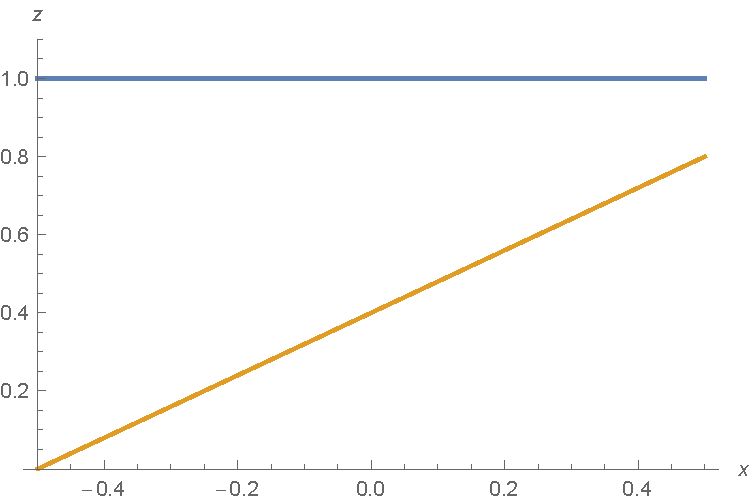
\includegraphics[width=\textwidth]{diagrams/bath-slope}
    \caption{Sloped.}
    \label{fig:bath-slope}
  \end{subfigure}
  \begin{subfigure}{0.45\textwidth}
    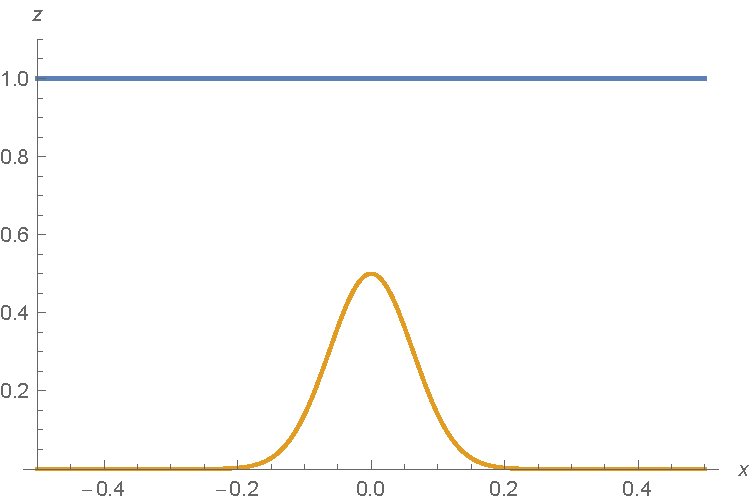
\includegraphics[width=\textwidth]{diagrams/bath-gaussian}
    \caption{Gaussian ridge.}
    \label{fig:bath-gaussian}
  \end{subfigure} \\
  \begin{subfigure}{0.45\textwidth}
    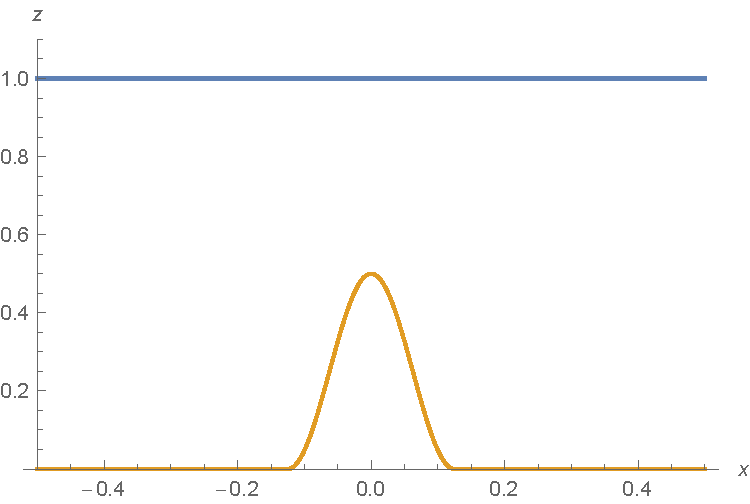
\includegraphics[width=\textwidth]{diagrams/bath-cosine}
    \caption{Cosine ridge.}
    \label{fig:bath-cosine}
  \end{subfigure}
  \begin{subfigure}{0.45\textwidth}
    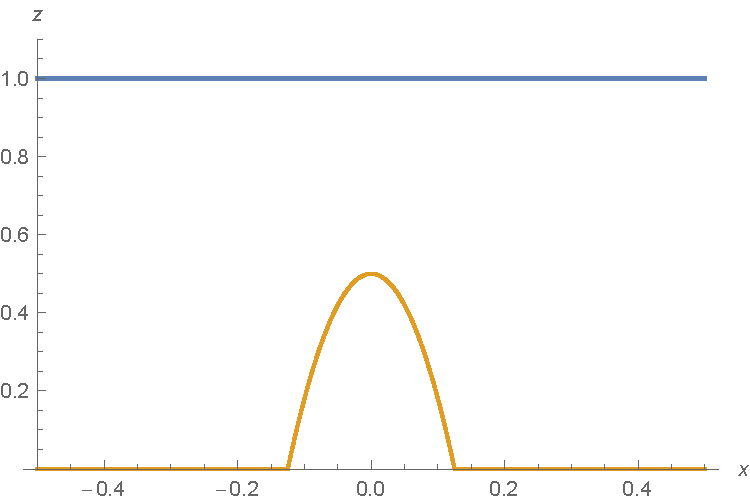
\includegraphics[width=\textwidth]{diagrams/bath-para-ridge}
    \caption{Parabolic ridge.}
    \label{fig:bath-para-ridge}
  \end{subfigure} \\
  \begin{subfigure}{0.45\textwidth}
    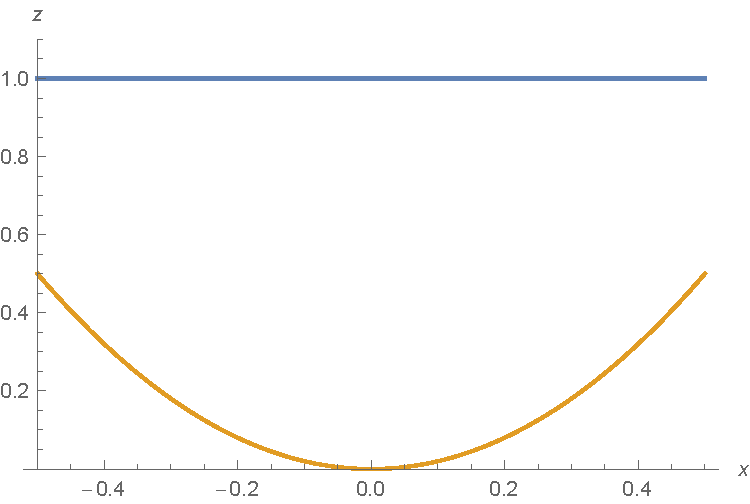
\includegraphics[width=\textwidth]{diagrams/bath-para-bowl}
    \caption{Parabolic bowl.}
    \label{fig:bath-para-bowl}
  \end{subfigure}
  \begin{subfigure}{0.45\textwidth}
    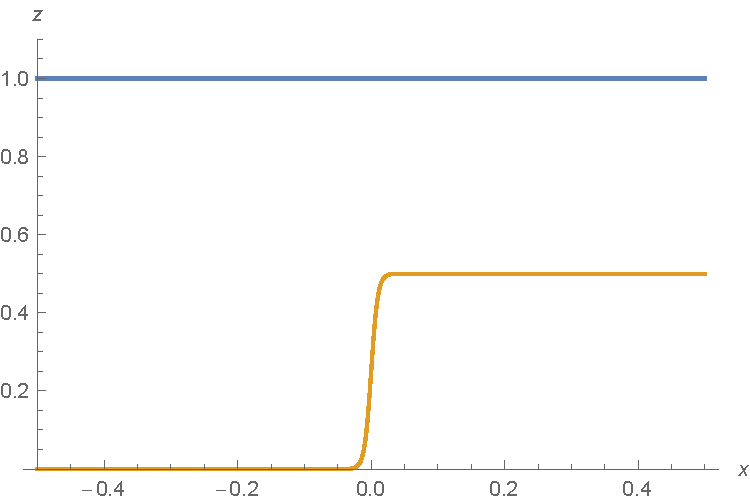
\includegraphics[width=\textwidth]{diagrams/bath-cliff}
    \caption{Cliff.}
    \label{fig:bath-cliff}
  \end{subfigure}
  \caption{Supported bathymetry profiles. Flat profile, $B = 0$, not depicted. Blue lines are still water level, $h_s = 1$, shown for scale. Orange lines are bathymetry.}
  \label{fig:bathymetries}
\end{figure}

These profiles are discretised by evaluating them on the cell edges and then averaging each cell's edge values to estimate the bathymetry at the cell centres, as required for the LeVeque solver. The other solvers do not impose any condition on the discretisation, so this scheme was used for all solvers.

The three ridge profiles may seem very similar qualitatively, but have been included for different reasons. The cosine ridge and parabolic ridge have compact support, which means that the regions of the domain affected by the bathymetry can be clearly distinguished from those which are not. Likewise, when waves travel across the ridge, it is clear at which time step the wave is first affected by the ridge. The difference between them is that the cosine ridge has a continuous derivative, while the parabola is not differentiable at $|x| = \frac{1}{8}$.

The Gaussian ridge does not have compact support but is still valuable, because this profile exactly matches the surface profile of the geostrophic equilibrium chosen (see below). By using the same profile for both water surface and bathymetry, the flux terms vanish completely (since $h$ becomes a constant), and the two source terms balance each other. This balance does not seem be addressed usually, presumably because a naive unbalanced method with source split will still be well-balanced with respect to the source terms themselves (as they are computed in the same step). However, it is worth verifying whether this balance is still preserved for methods which modify how source terms are treated.

Bathymetries with non-zero slope at the domain boundaries (i.e. sloped bathymetry and the parabolic bowl) were are a good test for the chosen boundary conditions.

Independently of the bathymetry profile, one of five initial conditions can be chosen. The framework takes into account the chosen bathymetry when calculating the initial values of $\vb q$. The supported initial conditions are the following:

\begin{itemize}
  \item Still water. Defined by $h_s = 1$, $u = v = 0$. Hence, the conserved variables are chosen to be $h = 1 - B$, $hu = hv = 0$. This is what is shown in Figs.~\ref{fig:bathymetries}.
  \item Wave through still water. This system is mostly identical to the still water case, apart from a small perturbation near one edge of the domain, such that $h_s = 1.05$ for $|x + 0.35| < 0.05$, and $h_s = 1$ otherwise. The basic behaviour is that the perturbation separates into two waves, one of which leaves the domain to the left and one of which traverses the domain and, in particular, the bathymetry where it may be partially reflected. The exact dynamics (especially in the presence of the Coriolis term) are more complicated, but this system allows a single wave to be studied in isolation. As an example, Fig.~\ref{fig:init_wave} shows the system for the cosine ridge.
  \item Geostrophic equilibrium. The surface level is fixed at $h_s = 1 + \frac{1}{2} \exp (-128 x^2)$, such that $h$ is chosen as $h_s - B$. Furthermore, $hu = 0$ and $hv$ is determined by Eq.~\ref{eq:geo_eq}. This system requires $K \neq 0$. Figs.~\ref{fig:init_geo} show this initial condition for the flat and cliff bathymetries and several values of $K$. Note that $hv$ depends both on the bathymetry and on $K$.
  \item Wave through geostrophic equilibrium. This is essentially a linear combination of the previous two systems. First, the geostrophic equilibrium is determined, and then a height perturbation of magnitude $0.05$ is added to the interval $x \in [-0.4, -0.3]$. $hv$ is unchanged from the geostrophic equilibrium. Fig.~\ref{fig:init_geo_wave} shows the initial water level for the parabolic bowl bathymetry.
  \item Uniform flow. Defined by $h_s = 1$, $u = U$, $v = 0$, where $U$ can be freely chosen. Unless the bathymetry is flat, this is not a steady state, but will settle into a steady system for many parameter combinations. $U$ can be used to choose between subcritical, transcritical and supercritical flows, as shown in \citet{esler2005steady}. Figs.~\ref{fig:init_flow} show initial momentum for two different bathymetries --- the initial water level is indistinguishable from the still water case, and $hv$ = 0 everywhere. Note that the momentum is not uniform, because $h$ varies.
\end{itemize}

\begin{figure}
  \centering
  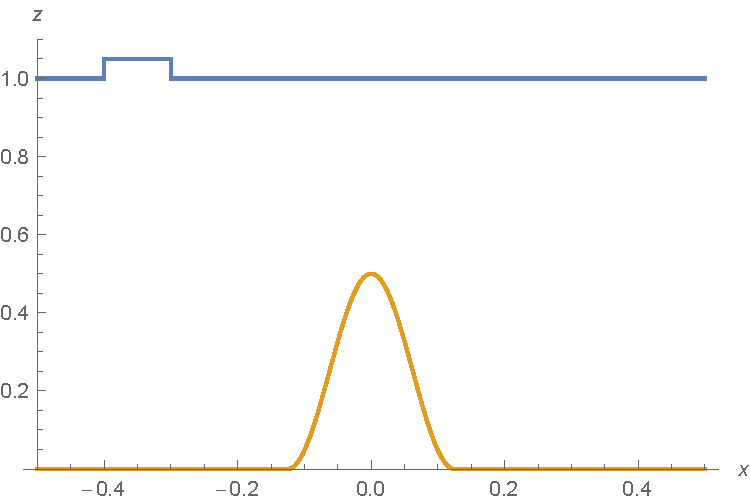
\includegraphics[width=0.45\textwidth]{diagrams/init-wave}
  \caption{Initial condition for ``wave through still water'' system and cosine bathymetry. Orange is the bathymetry profile, $B$. Blue is the initial water level, $h_s = h + B$.}
  \label{fig:init_wave}
\end{figure}

\begin{figure}
  \centering
  \begin{subfigure}{0.45\textwidth}
    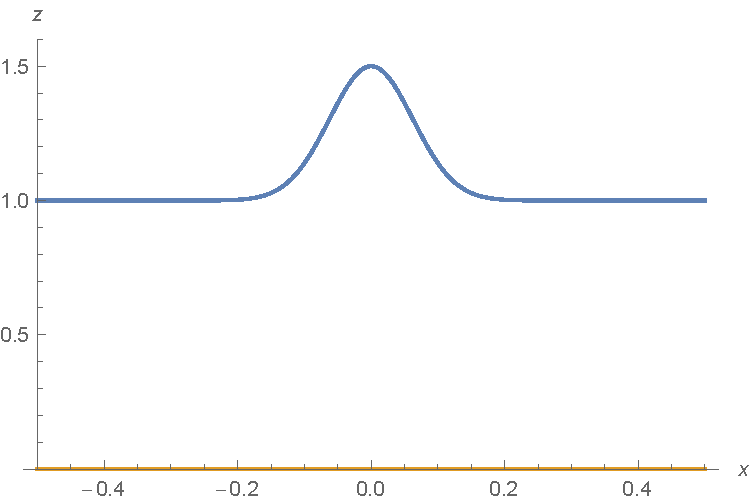
\includegraphics[width=\textwidth]{diagrams/init-geo-flat-h}
    \caption{Water level for flat bathymetry.}
    \label{fig:init-geo-flat-h}
  \end{subfigure}
  \begin{subfigure}{0.45\textwidth}
    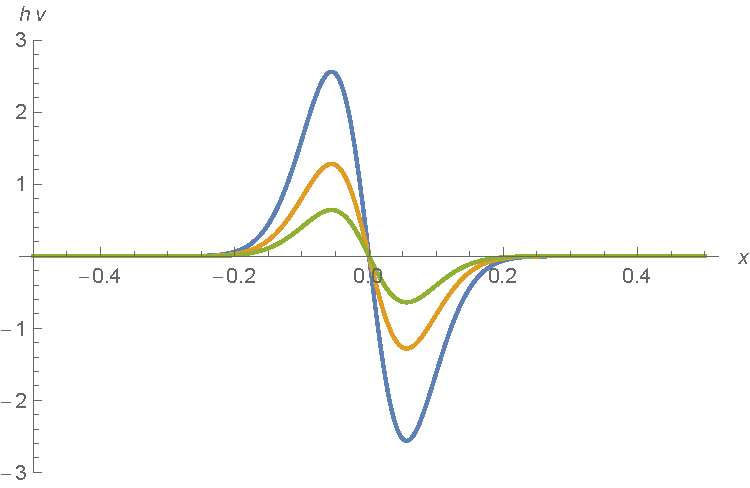
\includegraphics[width=\textwidth]{diagrams/init-geo-flat-hv}
    \caption{$y$-momentum for flat bathymetry.}
    \label{fig:init-geo-flat-hv}
  \end{subfigure} \\
  \begin{subfigure}{0.45\textwidth}
    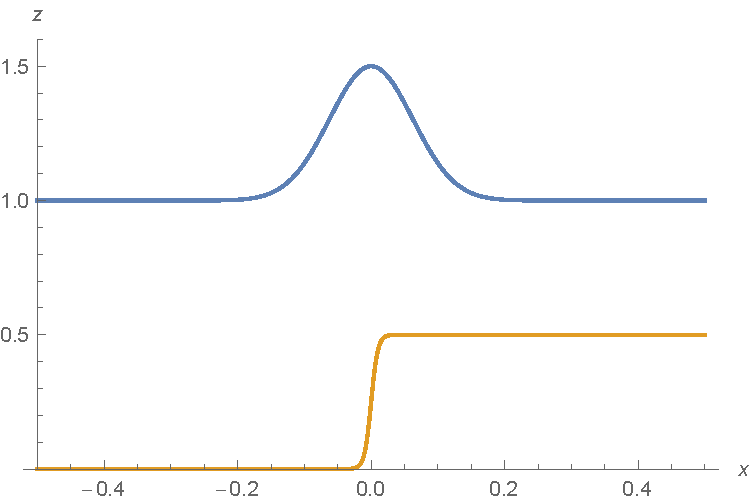
\includegraphics[width=\textwidth]{diagrams/init-geo-cliff-h}
    \caption{Water level for cliff bathymetry.}
    \label{fig:init-geo-cliff-h}
  \end{subfigure}
  \begin{subfigure}{0.45\textwidth}
    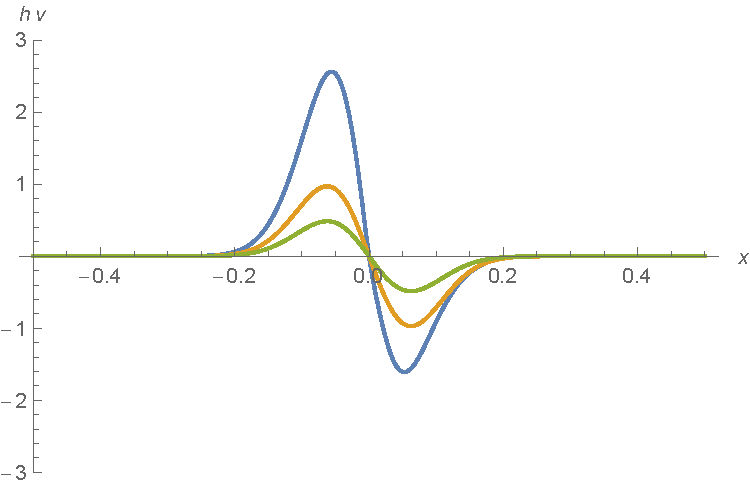
\includegraphics[width=\textwidth]{diagrams/init-geo-cliff-hv}
    \caption{$y$-momentum for cliff bathymetry.}
    \label{fig:init-geo-cliff-hv}
  \end{subfigure}
  \caption{Initial conditions for geostrophic equilibria for two bathymetry profiles. In the $hv$ plots, blue corresponds to $K = 2.5$, orange to $K = 5$ and green to $K = 10$.}
  \label{fig:init_geo}
\end{figure}

\begin{figure}
  \centering
  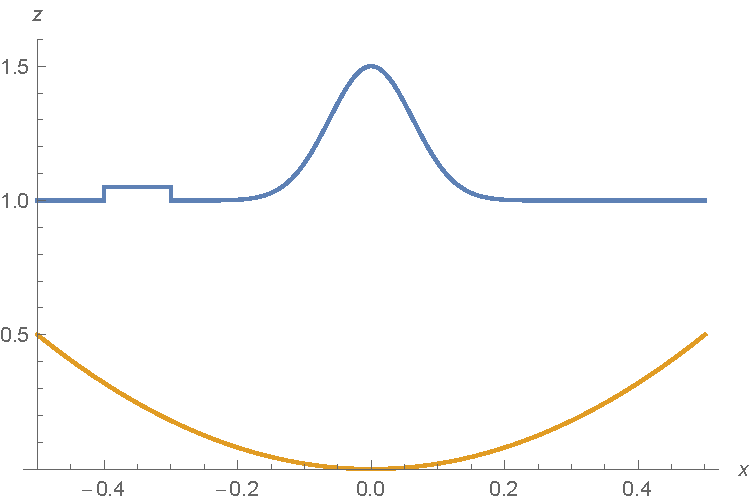
\includegraphics[width=0.45\textwidth]{diagrams/init-geo-wave}
  \caption{Initial condition for ``wave through geostrophic equilibrium'' system and parabolic bowl bathymetry. Orange is the bathymetry profile, $B$. Blue is the initial water level, $h_s = h + B$.}
  \label{fig:init_geo_wave}
\end{figure}

\begin{figure}
  \centering
  \begin{subfigure}{0.45\textwidth}
    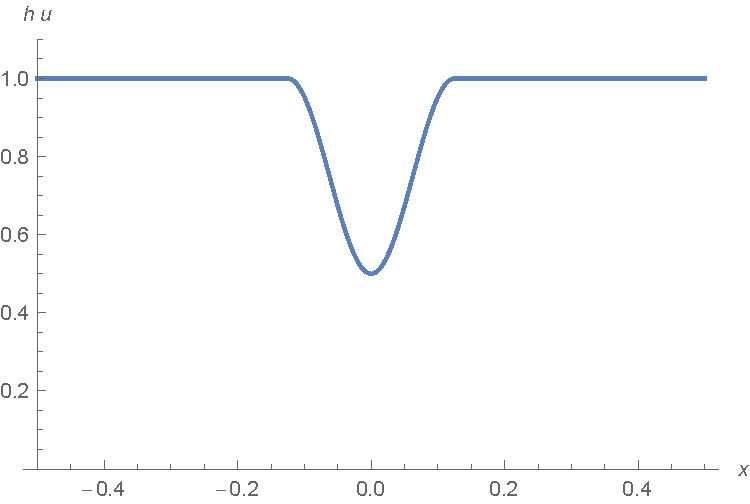
\includegraphics[width=\textwidth]{diagrams/init-steady-cosine}
    \caption{$x$-momentum for cosine ridge.}
    \label{fig:init-steady-cosine}
  \end{subfigure}
  \begin{subfigure}{0.45\textwidth}
    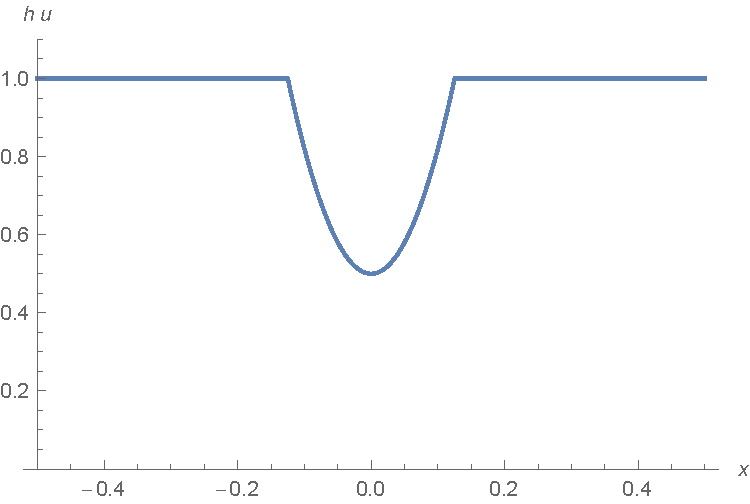
\includegraphics[width=\textwidth]{diagrams/init-steady-para}
    \caption{$x$-momentum for parabolic ridge.}
    \label{fig:init-steady-para}
  \end{subfigure}
  \caption{Initial conditions for uniform flow for two bathymetry profiles.}
  \label{fig:init_flow}
\end{figure}

\section{Notes on LeVeque Solver}

As mentioned in Section~\ref{sec:leveque}, a cubic needs to be solved to determine the size of the new Riemann problem at the cell centres. Two different approaches have been implement which can be chosen via a flag in the Fortran code:

\begin{itemize}
  \item As
\end{itemize}
%!TEX root = ../final-report.tex
\chapter{Results}
\label{ch:results}

This chapter presents results for the four solvers. For each of the five initial conditions, the solvers will be compared for a few representative bathymetries. Reference results were obtained using the unbalanced solver from Section~\ref{sec:roe} on a very fine grid of 10,000 cells. At the end, the execution time of the different solvers is compared as well.

\section{Still Water}



\begin{figure}
  \centering
  \begin{subfigure}{\textwidth}
    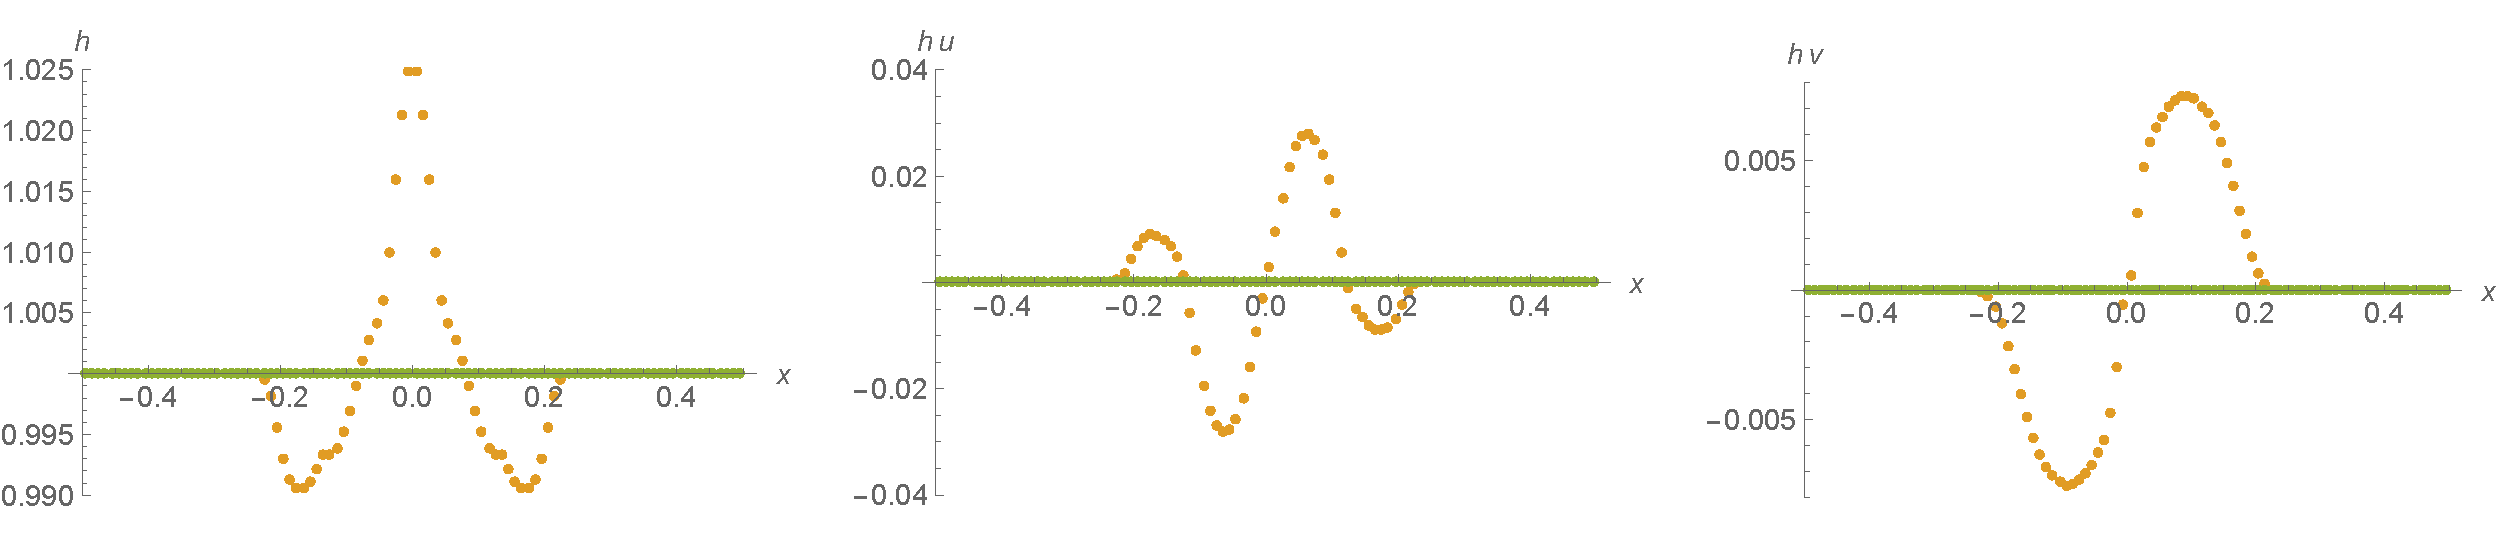
\includegraphics[width=\textwidth]{diagrams/results-still-1}
    \caption{$t = 0.1$}
    \label{fig:results-still-1}
  \end{subfigure} \\
  \begin{subfigure}{\textwidth}
    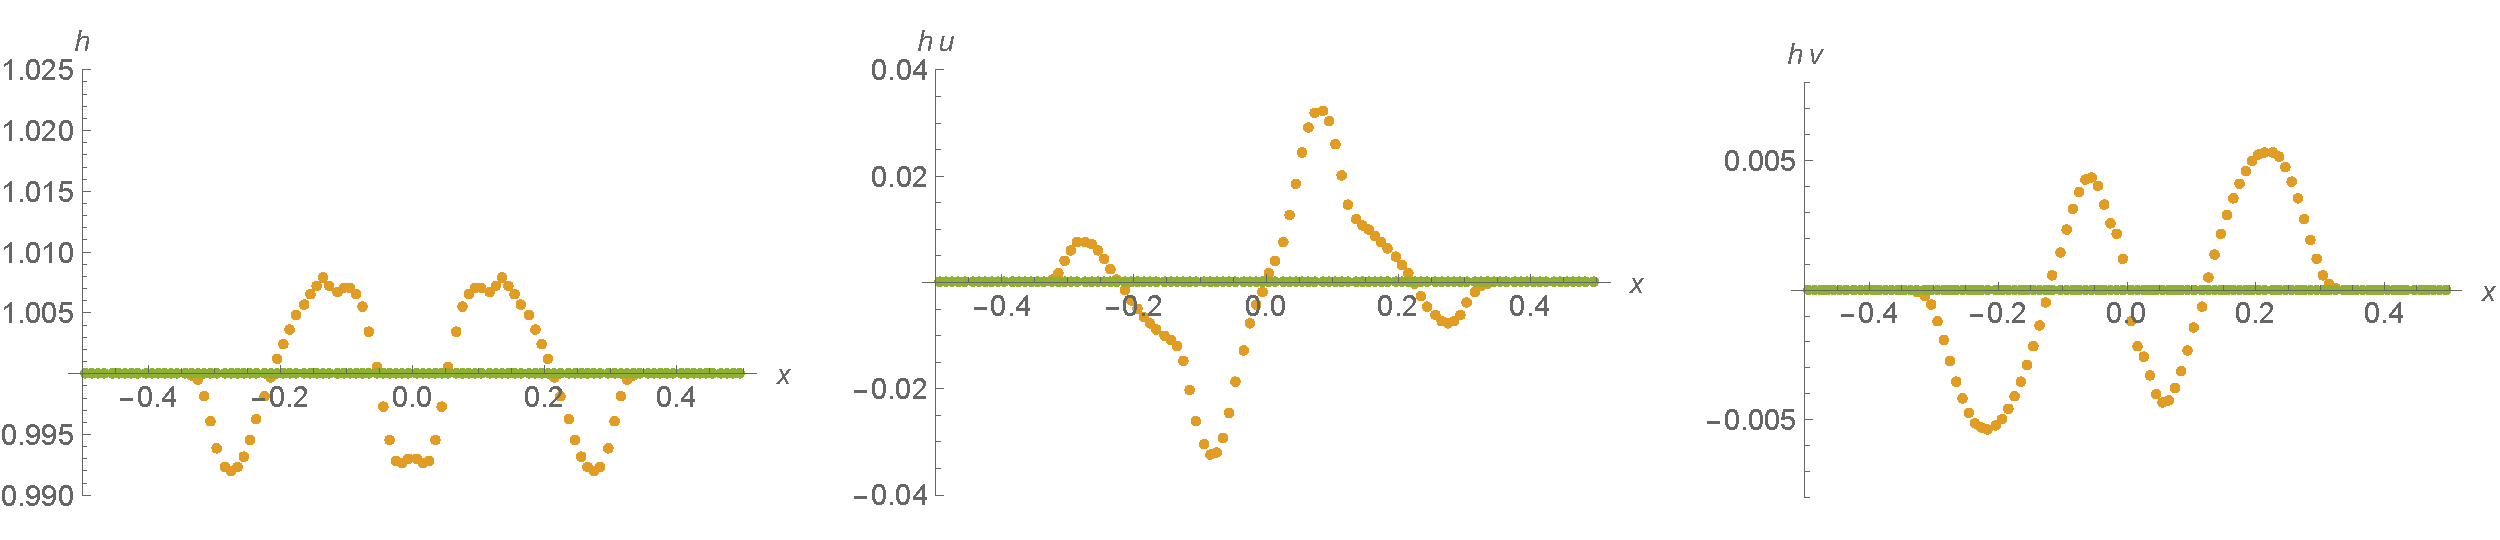
\includegraphics[width=\textwidth]{diagrams/results-still-2}
    \caption{$t = 0.2$}
    \label{fig:results-still-2}
  \end{subfigure} \\
  \begin{subfigure}{\textwidth}
    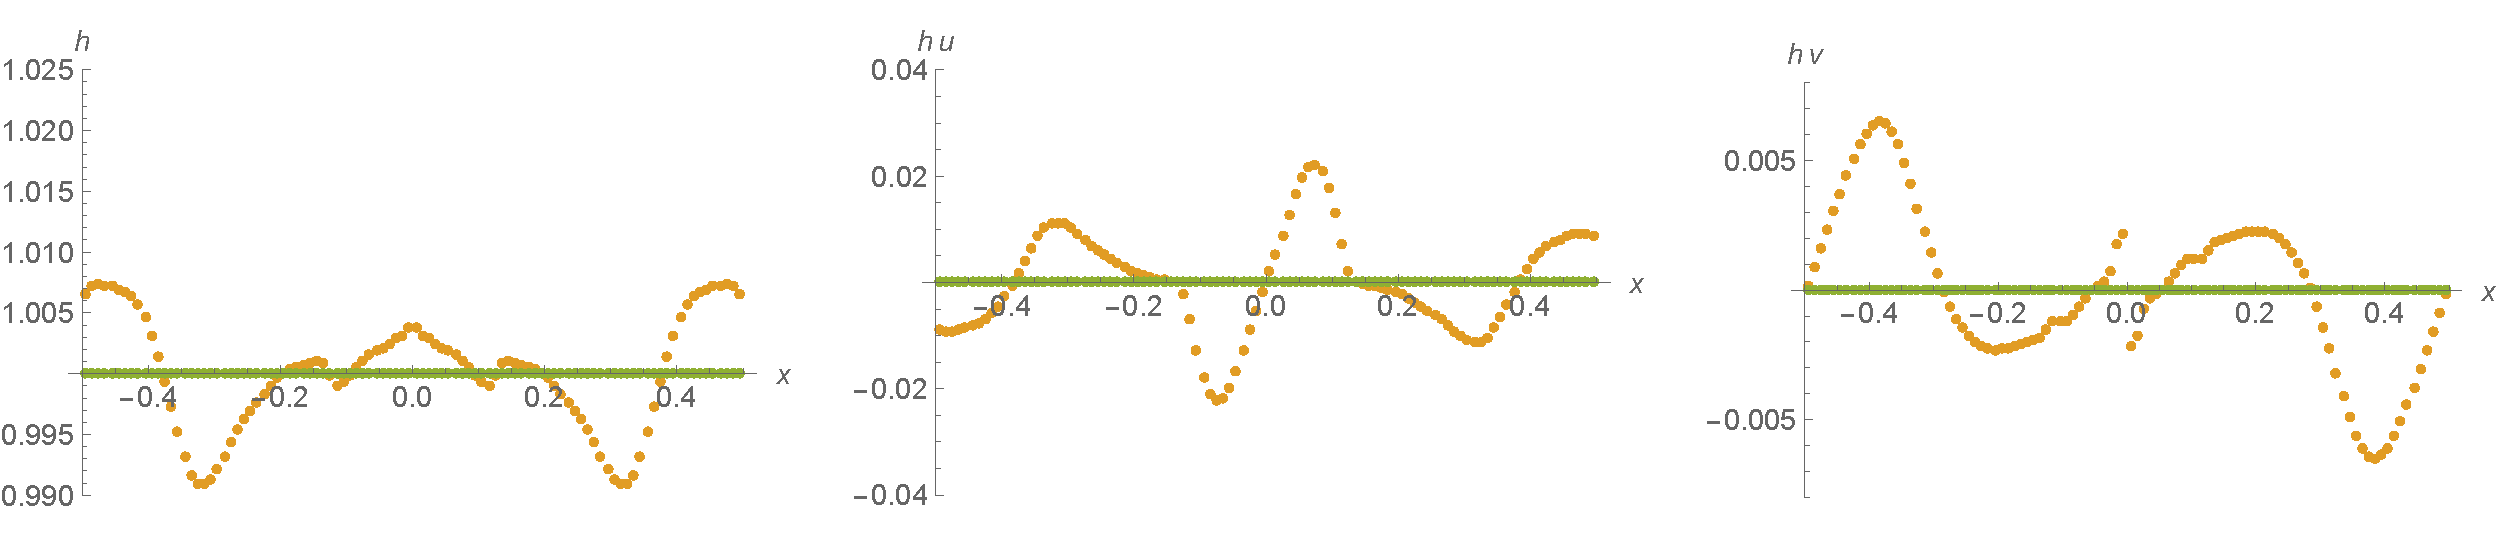
\includegraphics[width=\textwidth]{diagrams/results-still-5}
    \caption{$t = 0.5$}
    \label{fig:results-still-5}
  \end{subfigure} \\
  \begin{subfigure}{\textwidth}
    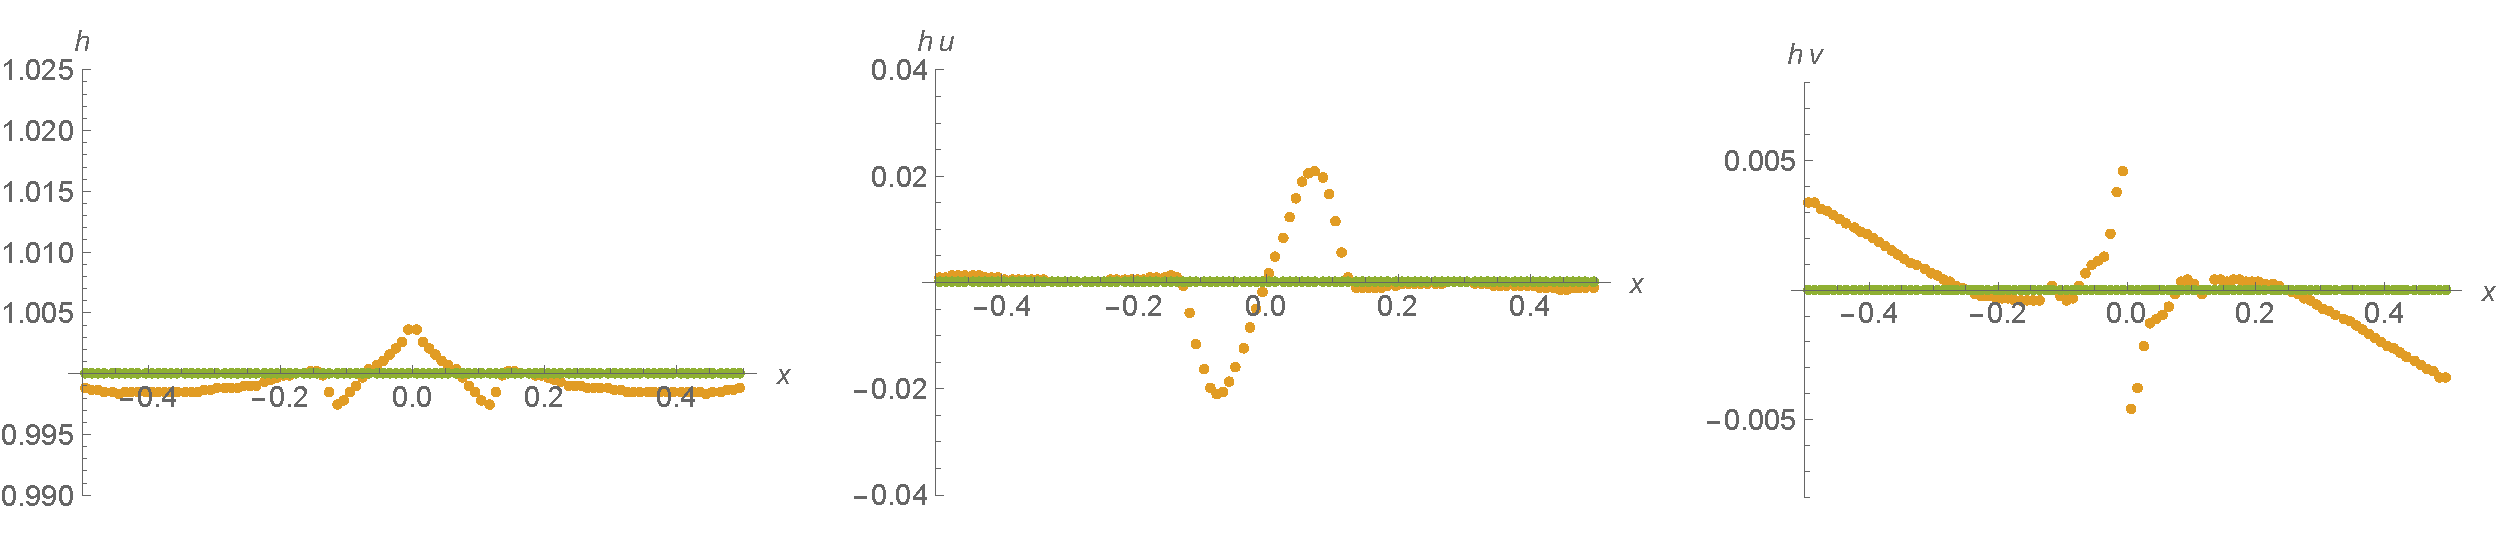
\includegraphics[width=\textwidth]{diagrams/results-still-10}
    \caption{$t = 1.0$}
    \label{fig:results-still-10}
  \end{subfigure}
  \caption{Results for still water over a cosine ridge. The exact solution is $h = 1$, $hu = hv = 0$ for all times. The orange data was obtained with the unbalanced solver over 100 grid cells.  The green data corresponds to any of the three balanced solvers.}
  \label{fig:results-still}
\end{figure}

\section{Wave through Still Water}

\section{Geostrophic Equilibrium}

\section{Wave through Geostrophic Equilibrium}

\section{Uniform Flow}

\section{Execution Time}

\begin{itemize}
  \item show how unbalanced method fails
  \item go through different methods, showing where they work and where they fail
\end{itemize}
%!TEX root = ../final-report.tex
\chapter{Conclusion}
\label{ch:conclusion}

\begin{itemize}
  \item quick recap
  \item pros and cons of the individual methods
  \item future work:
  \begin{itemize}
    \item derive more general Rogers solver for uniform flow
    \item what's with the growth of the still water solver for Gaussian geostrophic equilibrium?
    \item discrepancy with Rogers
    \item model additional effects/account for dry states
    \item look into methods that aren't Riemann problem based
    \item put more effort into choice of root for LeVeque solver
  \end{itemize}
\end{itemize}

\appendix

%!TEX root = ../final-report.tex
\chapter{Notes on method by Rogers et al.}
\label{ap:rogers}

In this report, the derivation of balanced solvers based on \citet{rogers2003mathematical} has been presented differently from what Rogers et al. have shown in their paper, and subsequently the result has been a different method.

The author initially attempted to implement the method as given in the paper, but this computed unphysical flows when the system was not in equilibrium, whereas the methods based on the author's theory do converge.

The discrepancy arises in the manipulation of Eq.~\ref{eq:rogers_discr}. Rogers at al. apply the chain rule directly to the $(\vb f(\vb q) - \vb f(\eq{\vb q}))_x$ term, obtaining $\pdv{\vb f'}{\vb q'}\vb q'_x$. Subsequently, they show that this deviatoric flux Jacobian is identical to the unmodified flux Jacobian $\vb A = \pdv{\vb f}{\vb q}$, obtaining the method

\begin{equation}
  \vb q'_t + \vb A \vb q'_x = \vb s'
\end{equation}

which differs from the author's method by the term $ - \vb A' \eq{\vb q}_x$ on the right-hand side.

While the result $\pdv{\vb f'}{\vb q'} = \pdv{\vb f}{\vb q}$ is undoubtedly correct, the first step seems to assume that $\vb f' = \vb f(\vb q) - \vb f(\eq{\vb q})$ is a function of $\vb q' = \vb q - \eq{\vb q}$ only --- otherwise the chain rule would yield additional terms. It is not obvious why this should be the case, such that there is no dependence on $\eq{\vb q}$ as well. This would be the most general case, since $\vb q$ itself can be decomposed into $\vb q'$ and $\eq{\vb q}$.

One can also go through this derivation without discarding this additional dependence:

\begin{align}
  \vb q'_t + \vb f'_x &= \vb s' \\
  \vb q'_t + \pdv{\vb f'}{\vb q'} \vb q'_x + \pdv{\vb f'}{\eq{\vb q}} \eq{\vb q}_x &= \vb s' \\
  \vb q'_t + \vb A \vb q'_x + \qty(\pdv{\vb f(\vb q)}{\eq{\vb q}} - \pdv{\vb f(\eq{\vb q})}{\eq{\vb q}}) \eq{\vb q}_x &= \vb s' \\
  \vb q'_t + \vb A \vb q'_x + \qty(\pdv{\vb f(\vb q)}{\vb q}\pdv{\vb q}{\eq{\vb q}} - \pdv{\vb f(\eq{\vb q})}{\eq{\vb q}}) \eq{\vb q}_x &= \vb s' \\
  \vb q'_t + \vb A \vb q'_x + \qty(\pdv{\vb f(\vb q)}{\vb q} - \pdv{\vb f(\eq{\vb q})}{\eq{\vb q}}) \eq{\vb q}_x &= \vb s' \\
  \vb q'_t + \vb A \vb q'_x + \qty(\vb A - \eq{\vb A}) \eq{\vb q}_x &= \vb s' \\
  \vb q'_t + \vb A \vb q'_x &= \vb s' - \vb A' \eq{\vb q}_x,
\end{align}

where the results $\pdv{\vb f'}{\vb q'} = \pdv{\vb f}{\vb q}$ and $\pdv{\vb q}{\eq{\vb q}} = 1$ have been used. This gives the same result as Eq.~\ref{eq:rogers_method}, including the additional source term.

The author has contacted Benedict Rogers and Alistair Borthwick about this discrepancy. However, while both of them replied very kindly, they do not seem to have addressed the problem with a justification for the initial manipulation --- from (3.9) to (3.10) in their paper.

However, Rogers at al. have obtained good results with their method, so it seems likely that there is simply a different underlying assumption in author's work than in theirs, which is accounted for by the additional source term. This should certainly be investigated further.


\addcontentsline{toc}{chapter}{Bibliography}
\bibliographystyle{plainnat}
\bibliography{../common/bibliography}

\end{document}
